%/**
% * @file tese.tex
% * @brief This file have the configuration parameters of Dr. Degree thesis.
% * @ingroup Documentation
% * @author $Author: rodcosta $
% * @version $Revision: 1.9 $
% * @date $Date: 2009/04/03 14:05:04 $
%**/
\documentclass[12pt,a4paper,oneside,final]{book}
\usepackage{listings}
\usepackage{verbatim}

%%% para vers\~{o}es parciais do dumento final utilizar:
%\documentclass[12pt,a4paper,draft]{book}
%\documentclass[12pt,a4paper,twoside,fleqn,draft]{book}
%%%%%%%%%%%%%%%%%%%%%%%%%%%%%%%%%%%%%%%%%%%%%%%%%%%%%%%%%%%%%%%%
%%% PREAMBULO DO DOCUMENTO COME\c{C}A AQUI
%\usepackage{natbib}
%\bibliographystyle{elsart-harv}
%inclui coisas da abnt
%\bibliographystyle{abntcite}
%\usepackage{hvfoat}

\usepackage{dissertacao}
\usepackage{multicol}
\usepackage{rotating}
%\usepackage{Fancyheader}
\usepackage{dissertacao_defs}
\usepackage[none]{hyphenat}
\usepackage[latin1]{inputenc}
\usepackage{rod_teste}
\usepackage{color}
\usepackage{pdfpages}
\usepackage{eso-pic}
\usepackage{everyshi}
%\usepackage{graphicx}
%\usepackage[alf]{abntcite}

\usepackage{multirow}
%\usepackage[small]{subfigure}
%\usepackage{multicol}
% \bibstyle{abnt-alf}
\usepackage{sidecap}
\usepackage{ifthen}
\usepackage{psfrag}
\newcommand{\titulo}{Um Novo Contador de N\'{u}cleos de Condensa\c{c}\~{a}o de Nuvens Baseado em T\'{e}cnicas de Vis\~{a}o Computacional}
\newcommand{\autor}{Francisco Geraldo de Melo Pinheiro}
\newcommand{\orientador}{Prof. Dr. Paulo C\'{e}sar Cortez}
\newcommand{\coorientador}{Prof. Dr. Jo\~{a}o C\'{e}sar Moura Mota}

\usepackage[breaklinks,pdftitle={\titulo},pdfauthor = {\autor}]{hyperref}
\newcommand{\alfref}{0}
\ifthenelse{\isundefined{\alfref}}{
\usepackage[square]{natbib}
}{
\usepackage[sort]{cite}
\usepackage[alf,abnt-and-type=e,abnt-full-initials=no,abnt-last-names=abnt,abnt-etal-list=0,abnt-etal-text = emph]{abntcite}
\newcommand{\citet}[1]{\citeonline{#1}}
}
\newcommand{\figref}[1]{Figura~\ref{#1}}
\newcommand{\fisgref}[1]{Figuras~\ref{#1}}
\newcommand{\equref}[1]{Equa\c{c}\~{a}o~\ref{#1}}
%\newcommand{\eqref}[1]{(\ref{#1})}

\newcommand{\secref}[1]{Se\c{c}\~{a}o~\ref{#1}}
\newcolumntype{Y}{>{\centering\arraybackslash}X}


\usepackage[dvips]{graphicx}
%\usepackage[portuges]{babel}
\usepackage[printonlyused]{acronym}
%\usepackage[final]{pdfpages}
%\usepackage{Fancyhdr}
%\bibliographystyle{IEEEtranPor}
% \includeonly{capa,agradecimentos}
% \includeonly{capa_externa,capa}
%%% PREAMBULO DO DOCUMENTO ACABA AQUI
%%%%%%%%%%%%%%%%%%%%%%%%%%%%%%%%%%%%%%%%%%%%%%%%%%%%%%%%%%%%%%%%

\usepackage{hvfloat}



\usepackage{longtable}
\usepackage{supertabular}
\usepackage{tabularx}
%\usepackage{listings}
\begin{document}
\newcommand{\membroa}{Prof. Dr. Jo\~{a}o Cesar Moura Mota \\ Co-orientador}
\newcommand{\membrob}{Prof. Dr. ???? \\ ????}
\newcommand{\membroc}{Prof. Dr. ???? \\ ????}
\newcommand{\membrod}{Prof. Dr. ???? \\ ????}
%padronizacao
\newcommand{\capitulo}{\chapter}
\newcommand{\secao}{\section}
\newcommand{\subsecao}{\subsection}
\DeclareGraphicsExtensions{.jpg,.pdf,.mps,.png}
%%%%%%%%%%%%%%%%%%%%%%%%%%%%%%%%%%%%%%%%%%%%%%%%%%%%%%%%%%%%%%%%
%%% CAPA

\thispagestyle{empty}%

\begin{center}
    
\includegraphics[width=2.5cm,bb=0 0 382 465]{figs/ufc.jpg} \\%
    \textsc{
    Universidade Federal do Cear\'{a} \\%
    Departamento de Engenharia de Teleinform\'{a}tica \\%
    Programa de P\'{o}s Gradua\c{c}\~{a}o em Engenharia de Teleinform\'{a}tica\\
    }
    \vspace{2.5 cm}%
%   {\normalsize    \textbf{Autor} \\%
%                     \textbf{Carlos H\'{e}racles Morais de Lima}} \\%
    {                \textbf{\autor}
    } \\%

    \null\vfill%%
    \vspace{.2cm}%
%        \textbf{Proposta de Tese submetida a Coordena\c{c}\~{a}o do Programa de P\'{o}s Gradua\c{c}\~{a}o em Engenharia de Teleinform\'{a}tica}\\
        {\Large         \textbf{\titulo}\\}



    \null\vfill%%
    \vspace{1 cm}%
    {\normalsize    \textsc{Fortaleza -- Cear\'{a} \\%
                            \monthname~2011 }}
\end{center}

\thispagestyle{empty}%

\begin{center}
    %
\includegraphics[width=2.5cm]{figs/ufc.jpg} \\%
%    \textsc{
%    Universidade Federal do Cear\'{a} \\%
%    Departamento de Engenharia de El\'{e}trica \\%
%    Programa de P\'{o}s Gradua\c{c}\~{a}o em Engenharia de Teleinform\'{a}tica\\
%    }
    \null\vfill%%
    \vspace{.25cm}%
    {\normalsize    \textbf{Autor:} \\%
                    \upshape{\autor}
                    }\\%

    \null\vfill%%
    \vspace{.25cm}%
    {\normalsize    \textbf{Orientador:} \\%
                    \upshape{\orientador}
                    } \\%
    \null\vfill%%
    \vspace{.25cm}%
%    {\normalsize    \textbf{Co-orientador:} \\%
%                    \upshape{\coorientador}
%                    } \\%

%    \null\vfill%%
    \vspace{.25cm}%
    {\large         \titulo\\}

    \null\vfill%%
    \vspace{.25cm}%
    \begin{tabularx}{\textwidth}{XX}

    \null\vfill \\
    &
    Monografia de Conclus\~{a}o de Curso apresentada \`{a} Coordena\c{c}\~{a}o do Curso de Gradua\c{c}\~{a}o em Engenharia de Teleinform\'{a}tica da Universidade Federal do Cear\'{a} como parte dos requisitos para obten\c{c}\~{a}o do grau de \textbf{Engenheiro de Teleinform\'{a}tica}. \\

    \end{tabularx}

    \null\vfill%%
    \vspace{.25cm}%

    {\normalsize    \textsc{Fortaleza -- Cear\'{a} \\%
                            \monthname~\the\year}}
\end{center}


%\thispagestyle{empty}%

\begin{center}
    %\includegraphics[width=2.5cm]{figs/UFC.eps} \\%
    \textsc{ \autor } \\
     \vspace{.5 cm} \textbf{ \titulo }     \\
\end{center}
    \vspace{.2 cm}
    Esta Tese foi julgada adequada para a obten\c{c}\~{a}o dos cr\'{e}ditos da disciplina Qualifica\c{c}\~{a}o de Doutorado II e aprovada em sua forma final pelo programa de P\'{o}s Gradua\c{c}\~{a}o em Engenharia de Teleinform\'{a}tica da Universidade Federal do Cear\'{a}.
    \assinatura{\autor}
    \vspace{0.2 cm}
     Banca Examinadora:
     \assinatura{\orientador \\ Orientador}
     \assinatura{\membroa}
     \assinatura{\membrob}
     \assinatura{\membroc}
     \assinatura{\membrod}
     \vspace{0.2 cm}%\null\vfill%%

\begin{center}
    {\normalsize    Fortaleza, \today}
\end{center}

\frontmatter \pagestyle{roman}
%%% DEDICAT\'{O}RIA
%\textbf{DEDICAT\'{O}RIA}
\thispagestyle{empty}%
\null\vfill
\begin{flushright}
Dedico este trabalho primeiramente a Deus, sem o qual nada na minha vida tem sentido. Dedico tamb�m � minha m�e Heronildes, meu pai Pl�nio, minha irm� Jamile, a toda minha fam�lia, � minha namorada Suelen e aos professores e amigos que caminharam junto a mim em algum momento da minha forma��o.
\end{flushright}

%\textbf{DEDICAT\'{O}RIA2}
\thispagestyle{empty}%
\null\vfill
\begin{flushright}
Ao meu pai Geraldo (em mem\'{o}ria) que mostrou, com exemplos, como ser filho, pai e amigo.
\`{A} minha m\~{a}e Filomena e \`{a} minha irm\~{a} Roseangela pela alegria contagiantes.
Aos meus irm\~{a}os Paulo Roberto e Simone Geraldine que mesmo distantes me incentivaram na realiza\c{c}\~{a}o deste trabalho.

\end{flushright}



%%%%%%%%%%%%%%%%%%%%%%%%%%%%%%%%%%%%%%%%%%%%%%%%%%%%%%%%%%%%%%%%
%%% AGRADECIMENTOS
\chapter*{Agradecimentos}
\label{CHP:ACKNOWLEDGMENT}%%
\thispagestyle{empty}
% \PARstartOne{A}{grade\c{c}o}
Quero expressar meus sinceros agradecimentos ao Professor Paulo C\'{e}sar Cortez pela sua inestim\'{a}vel orienta\c{c}\~{a}o, amizade, exemplo de dedica\c{c}\~{a}o \`{a} ci\^{e}ncia e que com sua experi\^{e}ncia e paci\^{e}ncia tornou poss\'{\i}vel a realiza\c{c}\~{a}o deste trabalho.

Ao Professor Jo\~{a}o C\'{e}sar Moura Mota, por seu constante incentivo, amizade, orienta\c{c}\~{a}o e que sempre apostou no meu desenvolvimento cient\'{\i}fico.

Ao Professor Carlos Jacinto de Oliveira que n\~{a}o economizou esfor\c{c}os no apoio ao desenvolvimento deste trabalho principalmente nas horas mais cr\'{\i}ticas, em especial no meu afastamento das atividades docentes na Universidade Estadual do Cear\'{a} bem como em meu est\'{a}gio no Max-Planck-Institute for Chemistry da Universidade de Mainz-Alemanha.

Ao Professor Stephan Borrmann, diretor do Departamento de Qu\'{\i}mica de Part\'{\i}culas do Max-Planck-Institute for Chemistry, por sua amizade e apoio decisivo para a realiza\c{c}\~{a}o dos experimentos.

N\~{a}o posso deixar de agradecer aos meus novos amigos Johannes Schneider, Julia Schmale, Paul Reitz, Friederike Freutel, Miklos Szakall, Frank Drewnick, St\'{e}phane Gallavardin, Johannes Fachinger, Katja Dzepina,  Karin Sulsky, Rosemarie Gross, pelo valioso apoio t\'{e}cnico, e que com amizade tornaram menos dif\'{\i}ceis os quatro meses que passei longe de minha casa.

Ao Professor Humberto Carmona, por sua amizade, incentivo e valiosas cr\'{\i}ticas e sugest\~{o}es na composi\c{c}\~{a}o deste trabalho.

Aos companheiros de doutorado do Laborat\'{o}rio de Teleinform\'{a}tica, John Hebert da Silva Felix, Auzuir Ripardo Alexandria  e Rodrigo Carvalho Sousa Costa, pelas sugest\~{o}es e ideias ao longo do desenvolvimento deste trabalho.

Ao Professor Gerson Paiva Almeida pelo apoio e sugest\~{o}es.

Ao amigo Manuel Pereira pelo incentivo, pelas suas ideias que demonstram toda a sua criatividade.

Aos professores do Colegiado do Curso de F\'{\i}sica da Universidade Estadual do Cear\'{a} que, com sacrif\'{\i}cio pr\'{o}prio, apoiaram este trabalho substituindo-me nas minhas tarefas docentes.

Ao Max-Planck-Institute for Chemistry pela oportunidade de desenvolver parte essencial do meu trabalho em seus laborat\'{o}rios.

\`{A} Funda\c{c}\~{a}o Cearense de Meteorologia e Recursos H\'{\i}dricos - FUNCEME e \`{a} Financiadora de Estudos e Projetos - FINEP pelo apoio financeiro no desenvolvimento do prot\'{o}tipo do CCNC-SDCC, objeto deste trabalho.

\`{A} Funda\c{c}\~{a}o Cearense de Apoio ao Desenvolvimento Cient\'{\i}fico e Tecnol\'{o}gico - FUNCAP pela bolsa concedida que possibilitou minha temporada no Max-Planck-Institute for Chemistry.

Aos meus pais, Geraldo Pinheiro e Filomena, que n\~{a}o mediram esfor\c{c}os na educa\c{c}\~{a}o de seus filhos.

\`{A} minha av\'{o}, Geralda (em mem\'{o}ria), pelo carinho e amor a mim dedicados. \\


%/
%/


A Deus por tudo. 
%\textbf{DEDICAT\'{O}RIA}
\thispagestyle{empty}%
\newpage
\null\vfill
\begin{flushright}
\emph{"Everything makes sense a bit at a time. But when you try to think of it all at once, it comes out wrong."}\\
Terry Pratchett
\end{flushright}
   \vspace{3.0cm}

%%\textbf{DEDICAT\'{O}RIA}
\thispagestyle{empty}%
\null\vfill
\begin{flushright}
Dedico este trabalho primeiramente a Deus, sem o qual nada na minha vida tem sentido. Dedico tamb�m � minha m�e Heronildes, meu pai Pl�nio, minha irm� Jamile, a toda minha fam�lia, � minha namorada Suelen e aos professores e amigos que caminharam junto a mim em algum momento da minha forma��o.
\end{flushright}

%%%%%%%%%%%%%%%%%%%%%%%%%%%%%%%%%%%%%%%%%%%%%%%%%%%%%%%%%%%%%%%%
%%% RESUMO
\chapter*{Resumo}
\label{CHP:RESUM0}%%
\thispagestyle{empty}




\PARstartOne{E}{sta} Tese prop\~{o}e um novo contador est\'{a}tico de n\'{u}cleos de condensa\c{c}\~{a}o de nuvens baseado em t\'{e}cnicas de vis\~{a}o computacional. O processo concebido nesse novo contador consiste na captura de uma amostra do ar atmosf\'{e}rico dentro de uma c\^{a}mara de nuvens est\'{a}tica supersaturada de vapor de \'{a}gua, produzindo got\'{\i}culas de \'{a}gua. Essas got\'{\i}culas, ao ca\'{\i}rem por gravidade, cruzam um feixe de LASER que define um volume de amostragem, tornando-as vis\'{\i}veis. Uma s\'{e}rie de imagens deste processo \'{e} digitalizada e processada para permitir a contagem das got\'{\i}culas presentes nesse volume de amostragem. Tais got\'{\i}culas s\~{a}o automaticamente contadas por um sistema de vis\~{a}o computacional composto por t\'{e}cnicas de binariza\c{c}\~{a}o por limiar, transformada de dist\^{a}ncia e transformada watershed. Esse volume de amostragem \'{e} calculado atrav\'{e}s de uma nova metodologia proposta nesta tese. Essa metodologia torna desnecess\'{a}ria a realiza\c{c}\~{a}o de complexos procedimentos de calibra\c{c}\~{a}o do contador desenvolvido bem como de outros similares. Um prot\'{o}tipo foi montado e experimentos baseados na compara\c{c}\~{a}o entre instrumentos foram realizados. Os resultados indicam que os procedimentos aplicados s\~{a}o adequados na determina\c{c}\~{a}o da concentra\c{c}\~{a}o dos n\'{u}cleos de condensa\c{c}\~{a}o de nuvens e que o equipamento desenvolvido pode ser usado em altas concentra\c{c}\~{o}es, situa\c{c}\~{a}o em que outros equipamentos equivalentes n\~{a}o s\~{a}o confi\'{a}veis, devido ao efeito da sobreposi\c{c}\~{a}o de got\'{\i}culas nas imagens analisadas. Al\'{e}m disso, a resolu\c{c}\~{a}o temporal foi significativamente melhorada e a intensa utiliza\c{c}\~{a}o da eletr\^{o}nica digital tamb\'{e}m permitiu a redu\c{c}\~{a}o de volume, de peso e de consumo de energia deste prot\'{o}tipo.



%\newline
%\newline
\noindent \textbf{Palavras-chaves:}  transformada \emph{watershed}; transformada de dist\^{a}ncia; processamento de imagens digitais; aerossol atmosf\'{e}rico; instrumenta\c{c}\~{a}o meteorol\'{o}gica.

\chapter*{Abstract}
\label{CHP:ABSTRACT}%%
\thispagestyle{empty}
\PARstartOne{T}{his} Thesis proposes a new static cloud condensation nuclei counter based on computer vision techniques. This process involves capturing a sample of atmospheric air inside a static cloud chamber supersaturated of water vapor, producing water droplets. These water droplets fall by gravity and cross a  laser beam, which define a sampling volume, making them visible. A serie of images of this process is digitalized and processed to determine the number of the droplets present in the sampling volume. These droplets are counted automatically by a computer vision system which uses three techniques: binarization by threshold, distance transform and watershed transform. The sampling volume is calculated using a new methodology, proposed in this thesis. This new methodology makes it unnecessary the use of sophisticated procedures to calibrate the developed counter. A prototype was assembled and experiments based on a comparison of those instruments were performed. The results indicate that the procedures developed are appropriate to determine the concentration of cloud condensation nuclei and that the developed device can be used in high concentrations, where equivalent products are unreliable due to the effect of overlapping droplets in the images analyzed. Moreover, the temporal resolution has been significantly improved and the intense use of digital electronics also allowed the reduction of volume, weight and power consumption of this prototype.

%\newline
%\newline
\noindent \textbf{Keywords:}watershed transform; distance transform; digital image processing; atmospheric aerosol; meteorological instrumentation.

%%%%%%%%%%%%%%%%%%%%%%%%%%%%%%%%%%%%%%%%%%%%%%%%%%%%%%%%%%%%%%%%


%%%%%%%%%%%%%%%%%%%%%%%%%%%%%%%%%%%%%%%%%%%%%%%%%%%%%%%%%%%%%%%%
%%% ABREVIA\c{C}\~{O}ES
\begin{singlespace}
    %%%%%%%%%%%%%%%%%%%%%%%%%%%%%%%%%%%%%%%%%%%%%%%%%%%%%%%%%%%%%%%%
    %%% \'{I}NDICE
    %\addtocontents{toc}{\noindent\protect\rule{\textwidth}{.2pt}\par}
    \tableofcontents%
    %%%%%%%%%%%%%%%%%%%%%%%%%%%%%%%%%%%%%%%%%%%%%%%%%%%%%%%%%%%%%%%%
    %%% LISTA DE FIGURAS
    \listoffigures%
    \addcontentsline{toc}{chapter}{Lista de Figuras}%
    %%%%%%%%%%%%%%%%%%%%%%%%%%%%%%%%%%%%%%%%%%%%%%%%%%%%%%%%%%%%%%%%
    %%% LISTA DE TABELAS
    \listoftables%
    \addcontentsline{toc}{chapter}{Lista de Tabelas}%
    %%%%%%%%%%%%%%%%%%%%%%%%%%%%%%%%%%%%%%%%%%%%%%%%%%%%%%%%%%%%%%%%
    %%% LISTA DE ALGORITMOS
    %    \listofalgorithms%
    %    \addcontentsline{toc}{chapter}{Lista de Algoritmos}%
     %\addtocontents{toc}{\noindent\protect\rule{\textwidth}{.2pt}\par}
    %%%%%%%%
    %%%% NOTA\c{C}\^{A}O
%    \addcontentsline{toc}{chapter}{Lista de S\'{\i}mbolos}%
%    \chapter*{Lista de S\'{\i}mbolos}%%
%    \LTXtable{\textwidth}{pretexto/simbolos}%%
%    \newpage
%    \addcontentsline{toc}{chapter}{Lista de Siglas}%
%    \chapter*{Lista de Siglas}%%
 %   \begin{acronym}[CAMshift]

\acro{Camshift}[CAMShift]{\emph{Continuously Adaptive Mean Shift}}

\acro{CCF}{Fun\c{c}\~{a}o de Correla\c{c}\~{a}o Cruzada \acroextra{(\emph{Cross-Correlation Function})}}

\acro{CVIU}{\acroextra{Revisa de Vis\~{a}o Computacional e Compreens\~{a}o de Imagem (} \emph{Journal of Computer Vision and Image Understanding}\acroextra{)}}

\acro{DT}{Diferencia\c{c}\~{a}o Temporal}

\acro{fop}[FO]{Fluxo \'{O}ptico}

\acro{fps}[FPS]{Quadros por Segundo \acroextra{(\emph{Frames per Second})}}

\acro{FPU}{Unidade de Ponto Flutuante\acroextra{(\emph{Floating Point Unit})}}

\acro{HSV}{Formato de Cor Tonalidade, Satura\c{c}\~{a}o e Brilho \acroextra{(\emph{Hue, Saturation e Brightness})}}

\acro{IHC}{Interfaces Homem-Computador}

\acro{LMS}{\emph{Least Mean Square} \acroextra{(M\'{\i}nimos Quadrados)}}

\acro{MPEG}{\acroextra{Padr\~{a}o de compress\~{a}o do} \emph{Moving Picture Experts Group}}

\acro{MSE}{Erro M\'{e}dio Quadr\'{a}tico \acroextra{(\emph{Mean Squared error})}}
\acro{GUI}{Interface Gr\'{a}fica do Usu\'{a}rio \acroextra{(\emph{Graphical User Interface})}}
\acro{PC}{Computador Pessoal \acroextra{(\emph{Personal Computer})}}

\acro{PDA}{Assistente Pessoal Digital \acroextra{(\emph{Personal Digital Assistant})}}

\acro{RITA}{Revista de Inform\'{a}tica e Teoria Aplicada}

\acro{RGB}{Formato de Cor \acroextra{Vermelho Verde Azul (}\emph{Red Green Blue} \acroextra{)}}

\acro{SAD}{Soma das Diferen\c{c}as Absolutas \acroextra{(\emph{Sum of Absolute Difference})}}

\acro{VC}{Vis\~{a}o Computacional}

\end{acronym} 
    %\LTXtable{\textwidth}{pretexto/siglas}%%
    %GATHER{pretexto/simbolos.tex}%%
    %GATHER{pretexto/siglas.tex}%%
\end{singlespace}

\pagestyle{capitulo} \setlength{\parskip}{1ex plus 0.5ex}
%%%%%%%%%%%%%%%%%%%%%%%%%%%%%%%%%%%%%%%%%%%%%%%%%%%%%%%%%%%%%%%%
%%% CAP\'{I}TULO 1: INTRODU\c{C}\~{A}O
\mainmatter
\include{ccnc_introducao/ccnc_introducao}
%%%%%%%%%%%%%%%%%%%%%%%%%%%%%%%%%%%%%%%%%%%%%%%%%%%%%%%%%%%%%%%
%%%% CAP\'{I}TULO 2: Aerossois
%\include{ccnc_aerossois/ccnc_aerossois}
%%%%%%%%%%%%%%%%%%%%%%%%%%%%%%%%%%%%%%%%%%%%%%%%%%%%%%%%%%%%%%%

%%%%%%%%%%%%%%%%%%%%%%%%%%%%%%%%%%%%%%%%%%%%%%%%%%%%%%%%%%%%%%%
%%%% CAP\'{I}TULO 3: CCNC_revis\~{a}o
\include{ccnc_revisao/ccnc_revisao}
%%\include{materiais}
%
%%%%%%%%%%%%%%%%%%%%%%%%%%%%%%%%%%%%%%%%%%%%%%%%%%%%%%%%%%%%%%%%%
%%%% CAP\'{I}TULO 3: Materiais e M\'{e}todos
\include{ccnc_sdcc/ccnc_metodologia}
%\include{chp3/cronograma}
%%%%%%%%%%%%%%%%%%%%%%%%%%%%%%%%%%%%%%%%%%%%%%%%%%%%%%%%%%%%%%%%%
%%%%%%% Capitulo 4: Bancada Geradora de Aeross\'{o}is
%\doublespacing
%% ------------------------------------------------------------------------- %%
\chapter{Bancada geradora de Aeross\'{o}is}
\label{cap:bancada}

O processo de gera\c{c}\~{a}o de aeross\'{o}is inicia-se em um compressor com sa\'{\i}da de ar filtrado. Em seguida, este ar filtrado passa por uma armadilha de \'{a}gua. Nesse ponto, o ar pressurizado, filtrado e seco \'{e} injetado no atomizador TSI3076 que esta acoplado a um reservat\'{o}rio, contendo uma solu\c{c}\~{a}o de sulfato de am\^{o}nia (NH$_4$)$_2$SO$_4$. Outras subst\^{a}ncias higrosc\'{o}picas podem ser utilizadas como por exemplo nitrato de am\^{o}nia NH$_4$NO$_3$, cloreto de s\'{o}dio NaCl e etc. Na sa\'{\i}da deste atomizador, tem-se os aeross\'{o}is propriamente dito, embora polidisperssivo e com uma umidade muito alta. A remo\c{c}\~{a}o da umidade \'{e} feita por um secador a base de silicagel.

Como o processo de condensa\c{c}\~{a}o do vapor de \'{a}gua \'{e} altamente dependente do tamanho do aerossol, ou seja , do tamanho do n\'{u}cleo de condensa\c{c}\~{a}o, exige-se um controle deste par\^{a}metro. Isto \'{e}, exige-se que o aerossol seja monodispersivo. Para tal, utiliza-se na sa\'{\i}da do secador um classificador eletrost\'{a}tico, que no caso \'{e} o TSI3080. Por fim, a medida da concentra\c{c}\~{a}o das part\'{\i}culas \'{e} feita por um contador de part\'{\i}culas condens\'{a}veis (CPC), no caso o TSI3025A.

O contador de part\'{\i}culas condens\'{a}veis  TSI3025A \'{e} capaz de medir aeross\'{o}is com um di\^{a}metro de 3nm at\'{e} 3$\mu$m numa faixa de concentra\c{c}\~{a}o  de 0 at\'{e} 9,99$\cdot$10$^{4}$ part\'{\i}culas / cm$^{3}$. Em condi\c{c}\~{o}es normais, seu sensor de part\'{\i}culas opera em uma atmosfera saturada de Butanol-1.  Essa caracter\'{\i}stica o torna sens\'{\i}vel,  n\~{a}o apenas aos aeross\'{o}is respons\'{a}veis pela forma\c{c}\~{a}o das nuvens e das chuvas, mas a qualquer aerossol. Por essa raz\~{a}o, no processo de compara\c{c}\~{a}o, normalmente se utiliza apenas aeross\'{o}is higrosc\'{o}picos (como por exemplo o sulfato de am\^{o}nia, nitrato de am\^{o}nia ou cloreto de s\'{o}dio) que s\~{a}o capazes de sensibilizar tanto o CCNC-SDCC quanto o CPC TSI3025A.


\begin{figure}[hbt]
\begin{center}
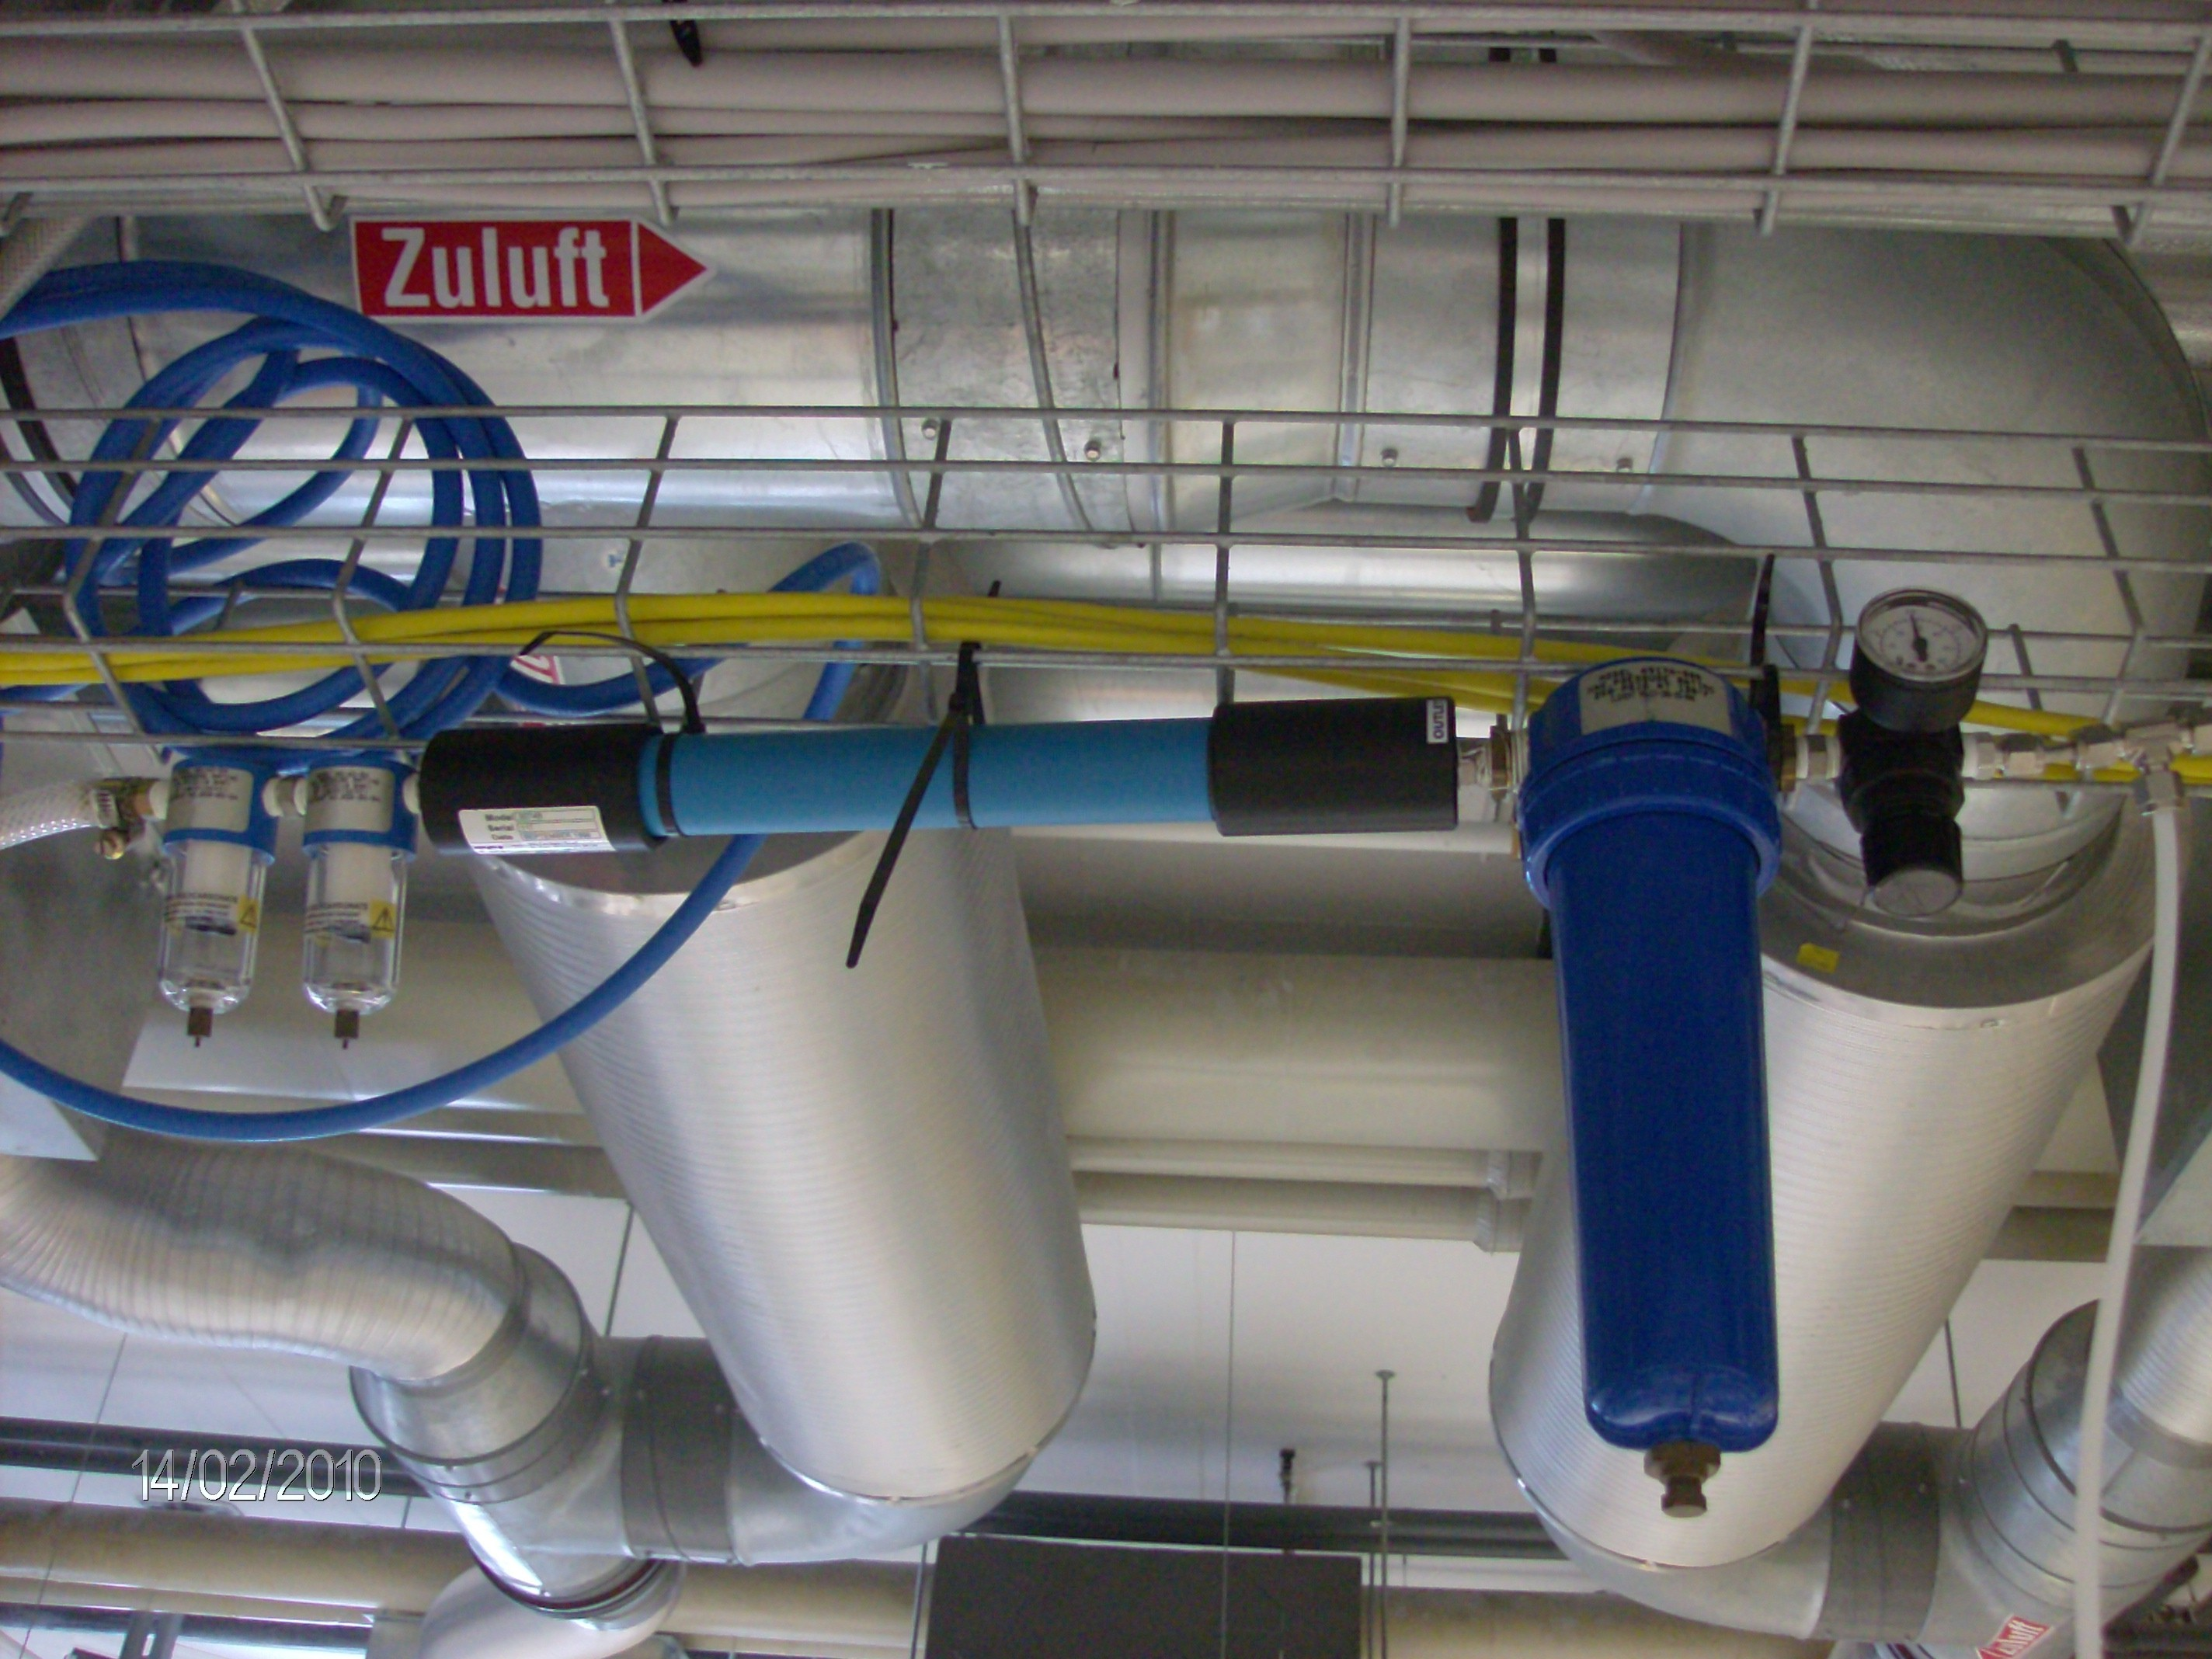
\includegraphics[scale=0.1]{eps/TSI3074FILTRO.eps}\\
\end{center}
\caption{\label{TSI3074FILTRO}\hspace{-0.1em} filtro para remo\c{c}\~{a}o de gotas de \'{o}leo, \'{a}gua e particulados (TSI3074B). }
\end{figure}

\begin{figure}[hbt]
\begin{center}
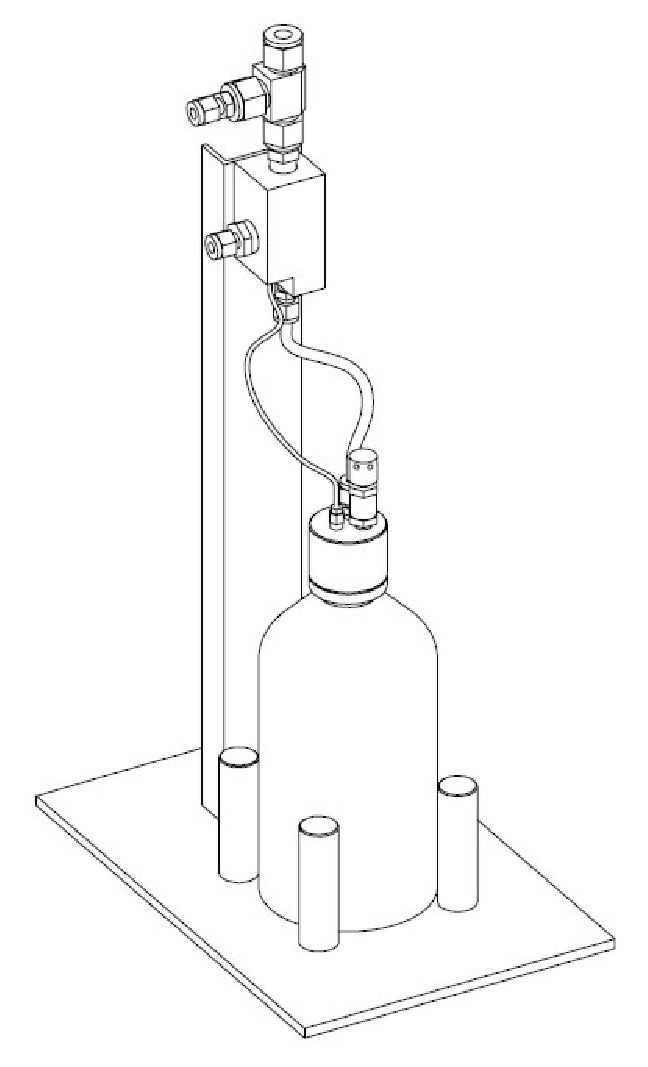
\includegraphics[scale=0.5]{eps/TSI3076ATOMIZADOR.eps}\\
\end{center}
\caption{\label{TSI3074FILTRO}\hspace{-0.1em} diagrama esquem\'{a}tico do atomizador (TSI3076).}
\end{figure}

\begin{figure}[hbt]
\begin{center}
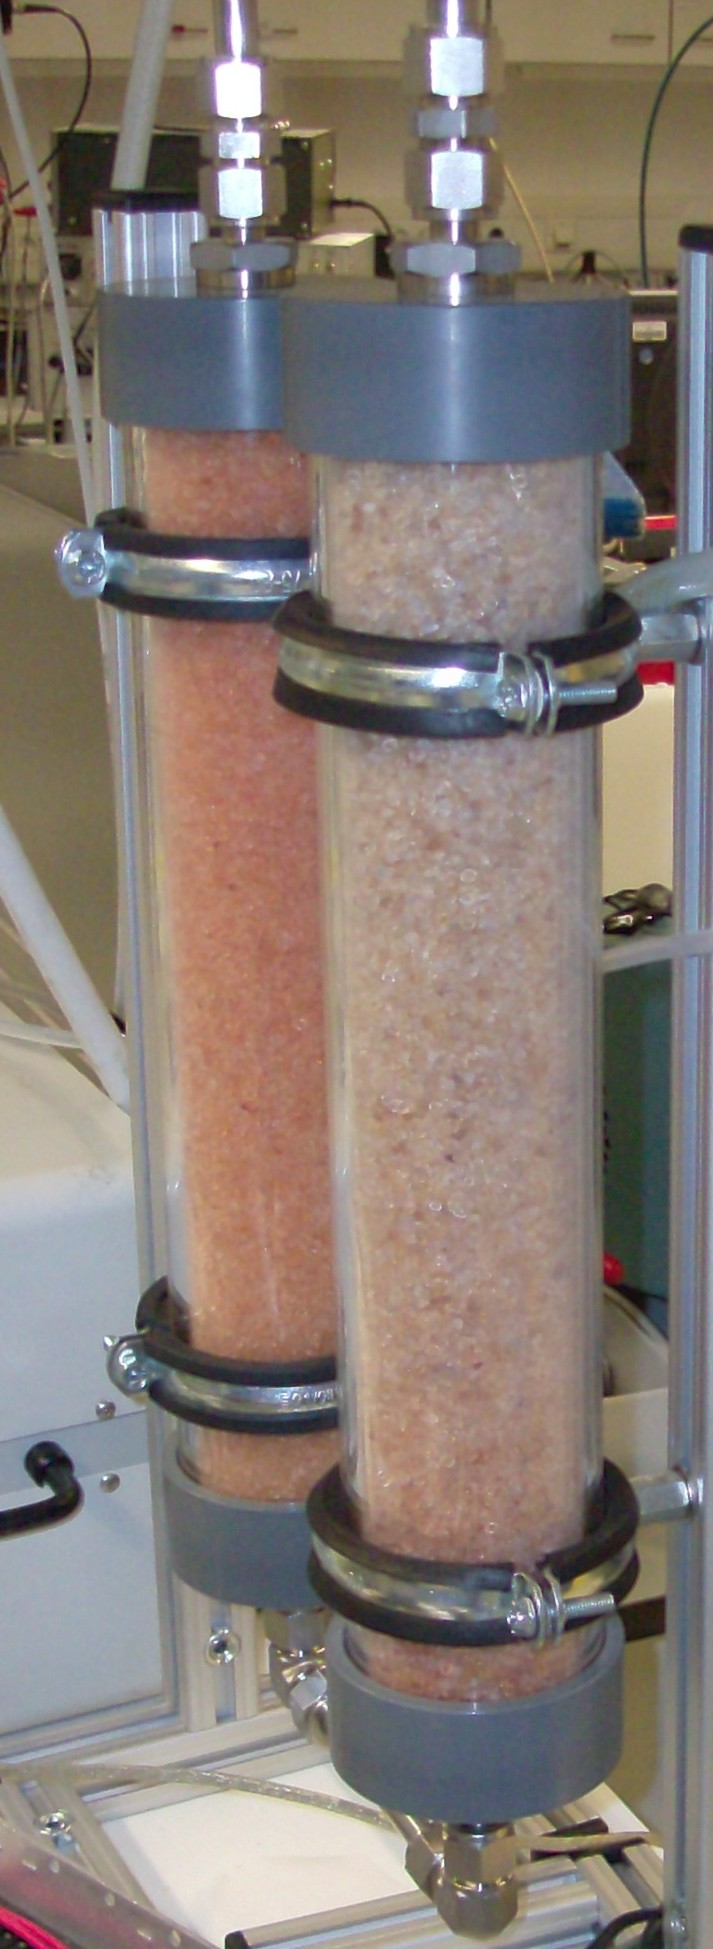
\includegraphics[scale=0.1]{eps/TSI3062SECADOR.eps}\\
\end{center}
\caption{\label{TSI3062SECADOR}\hspace{-0.1em} secador (TSI3062).}
\end{figure}



\begin{figure}[hbt]
\begin{center}
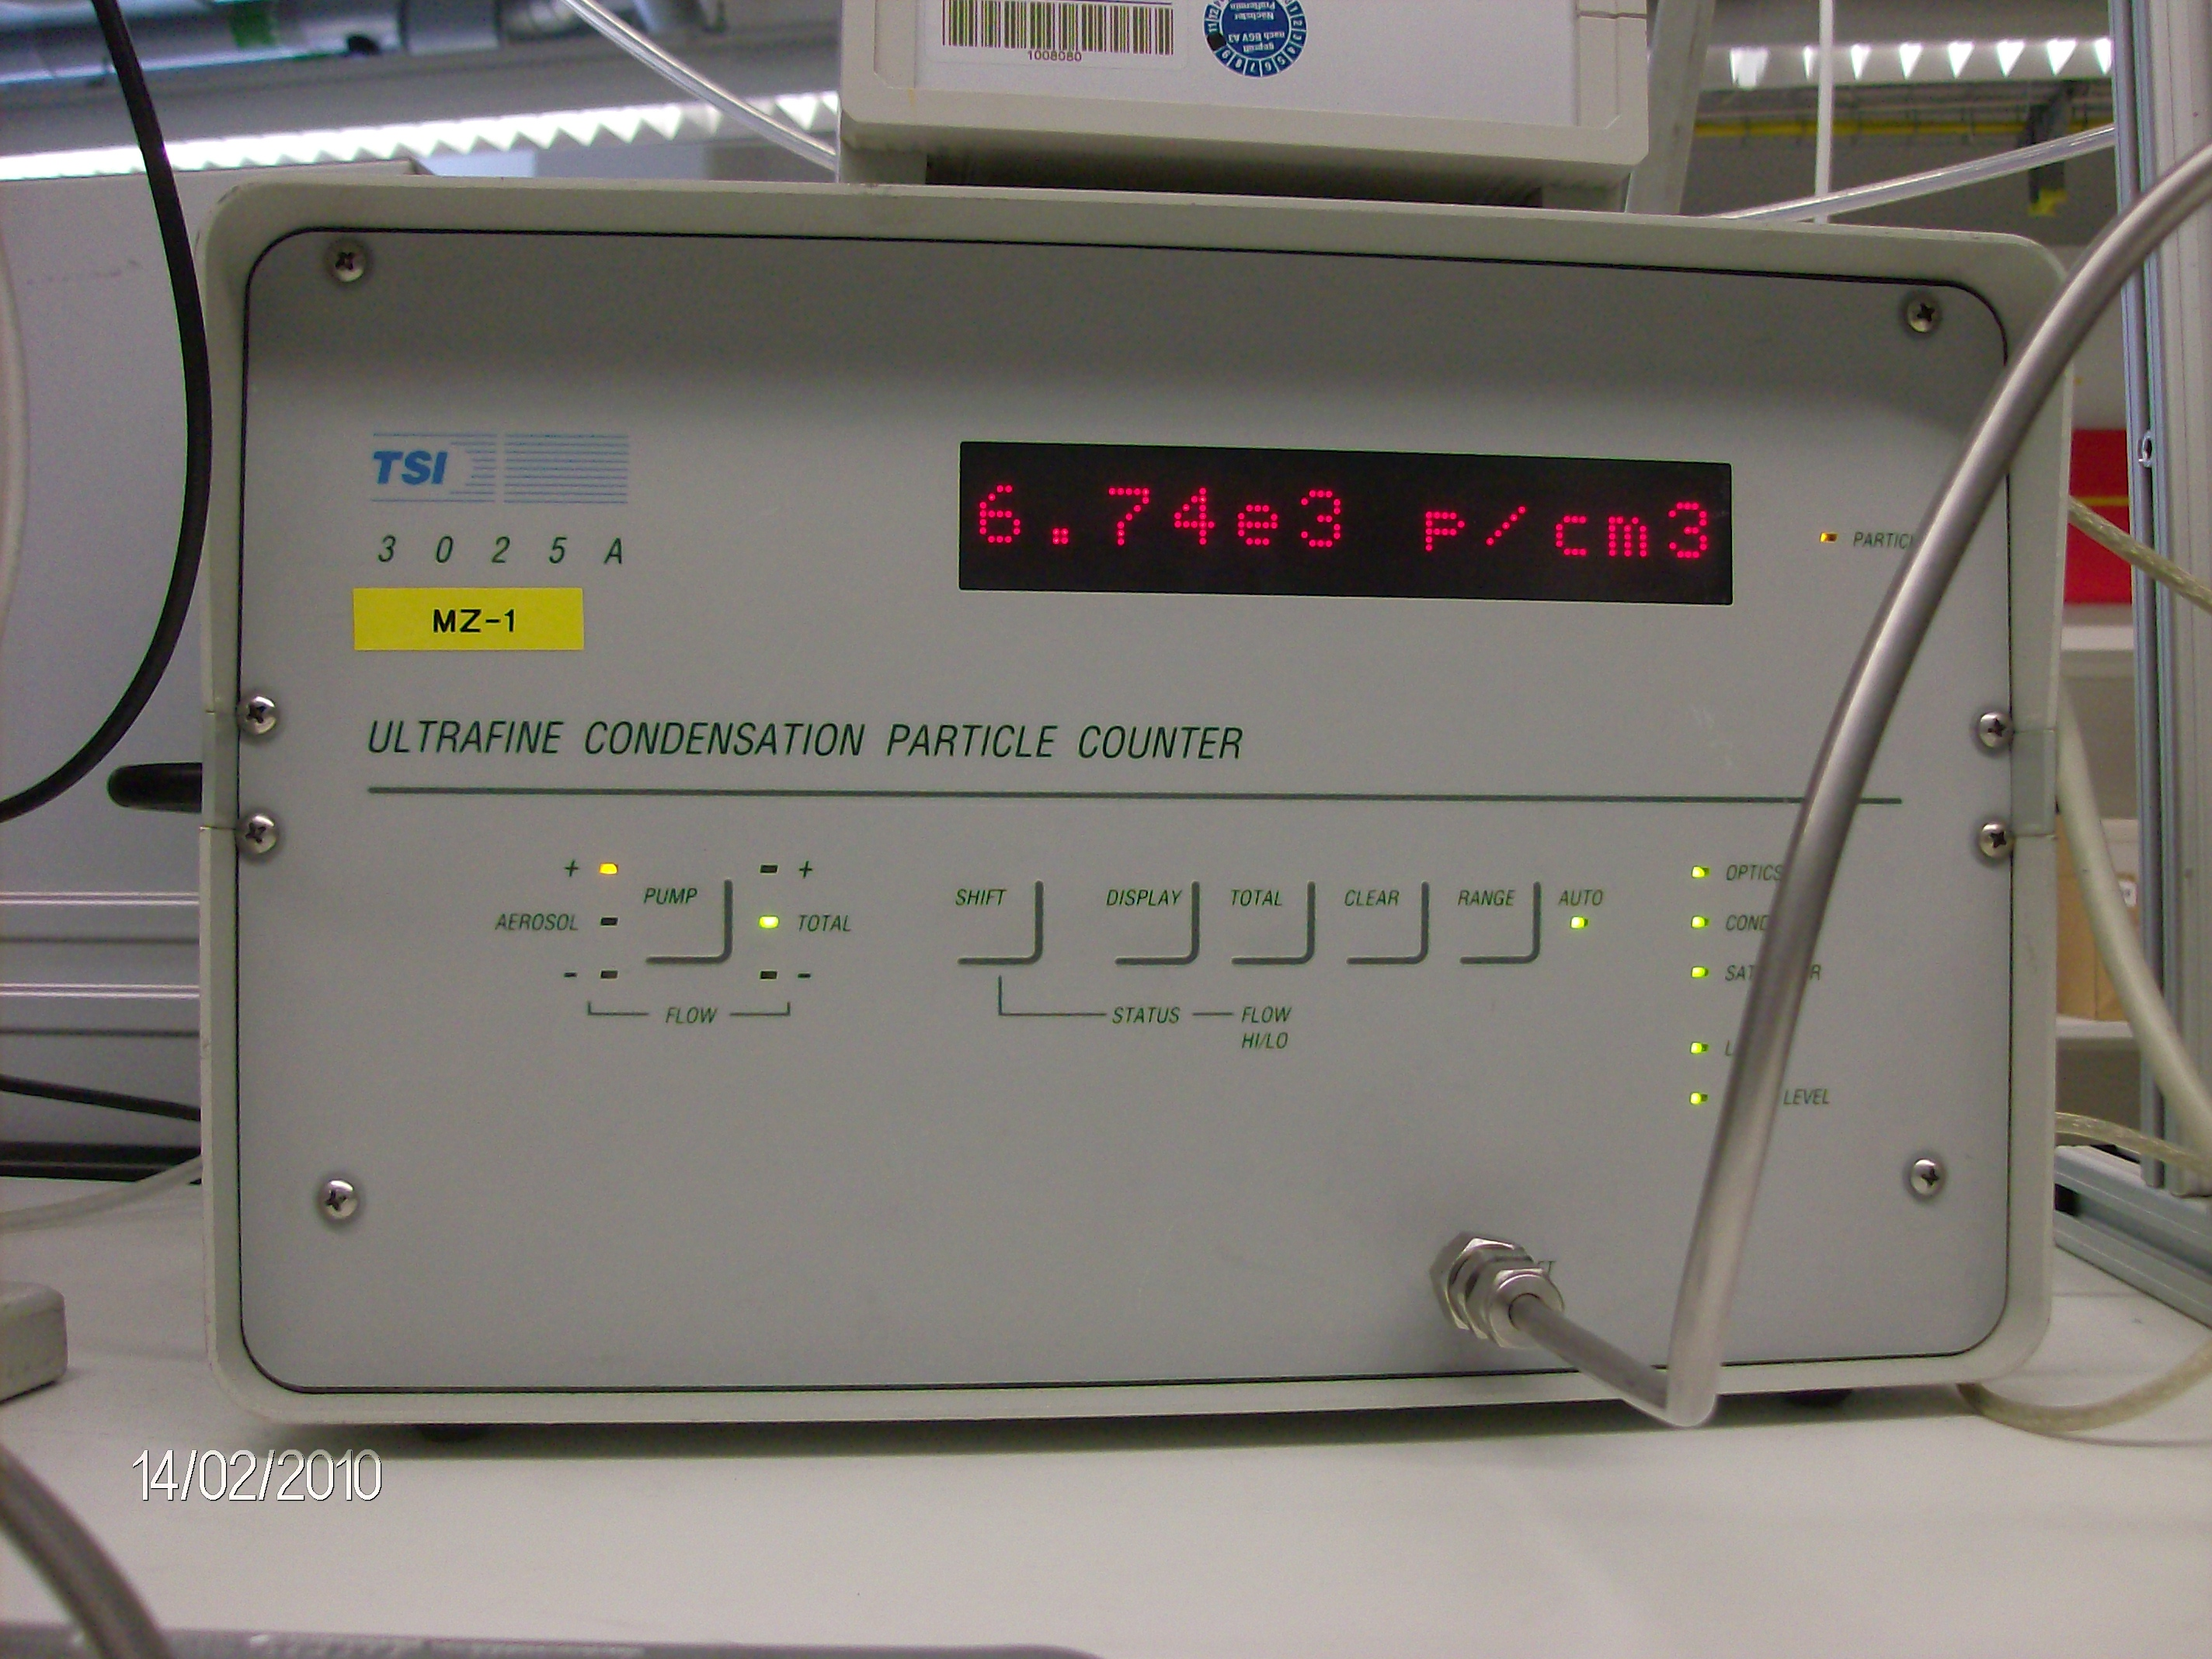
\includegraphics[scale=0.9]{eps/TSI3025CPC.eps}\\
\end{center}
\caption{\label{TSI3025CPC}\hspace{-0.1em} contador de part\'{\i}culas condens\'{a}veis  CPC (TSI 3025A).}
\end{figure}

\begin{figure}[hbt]
\begin{center}
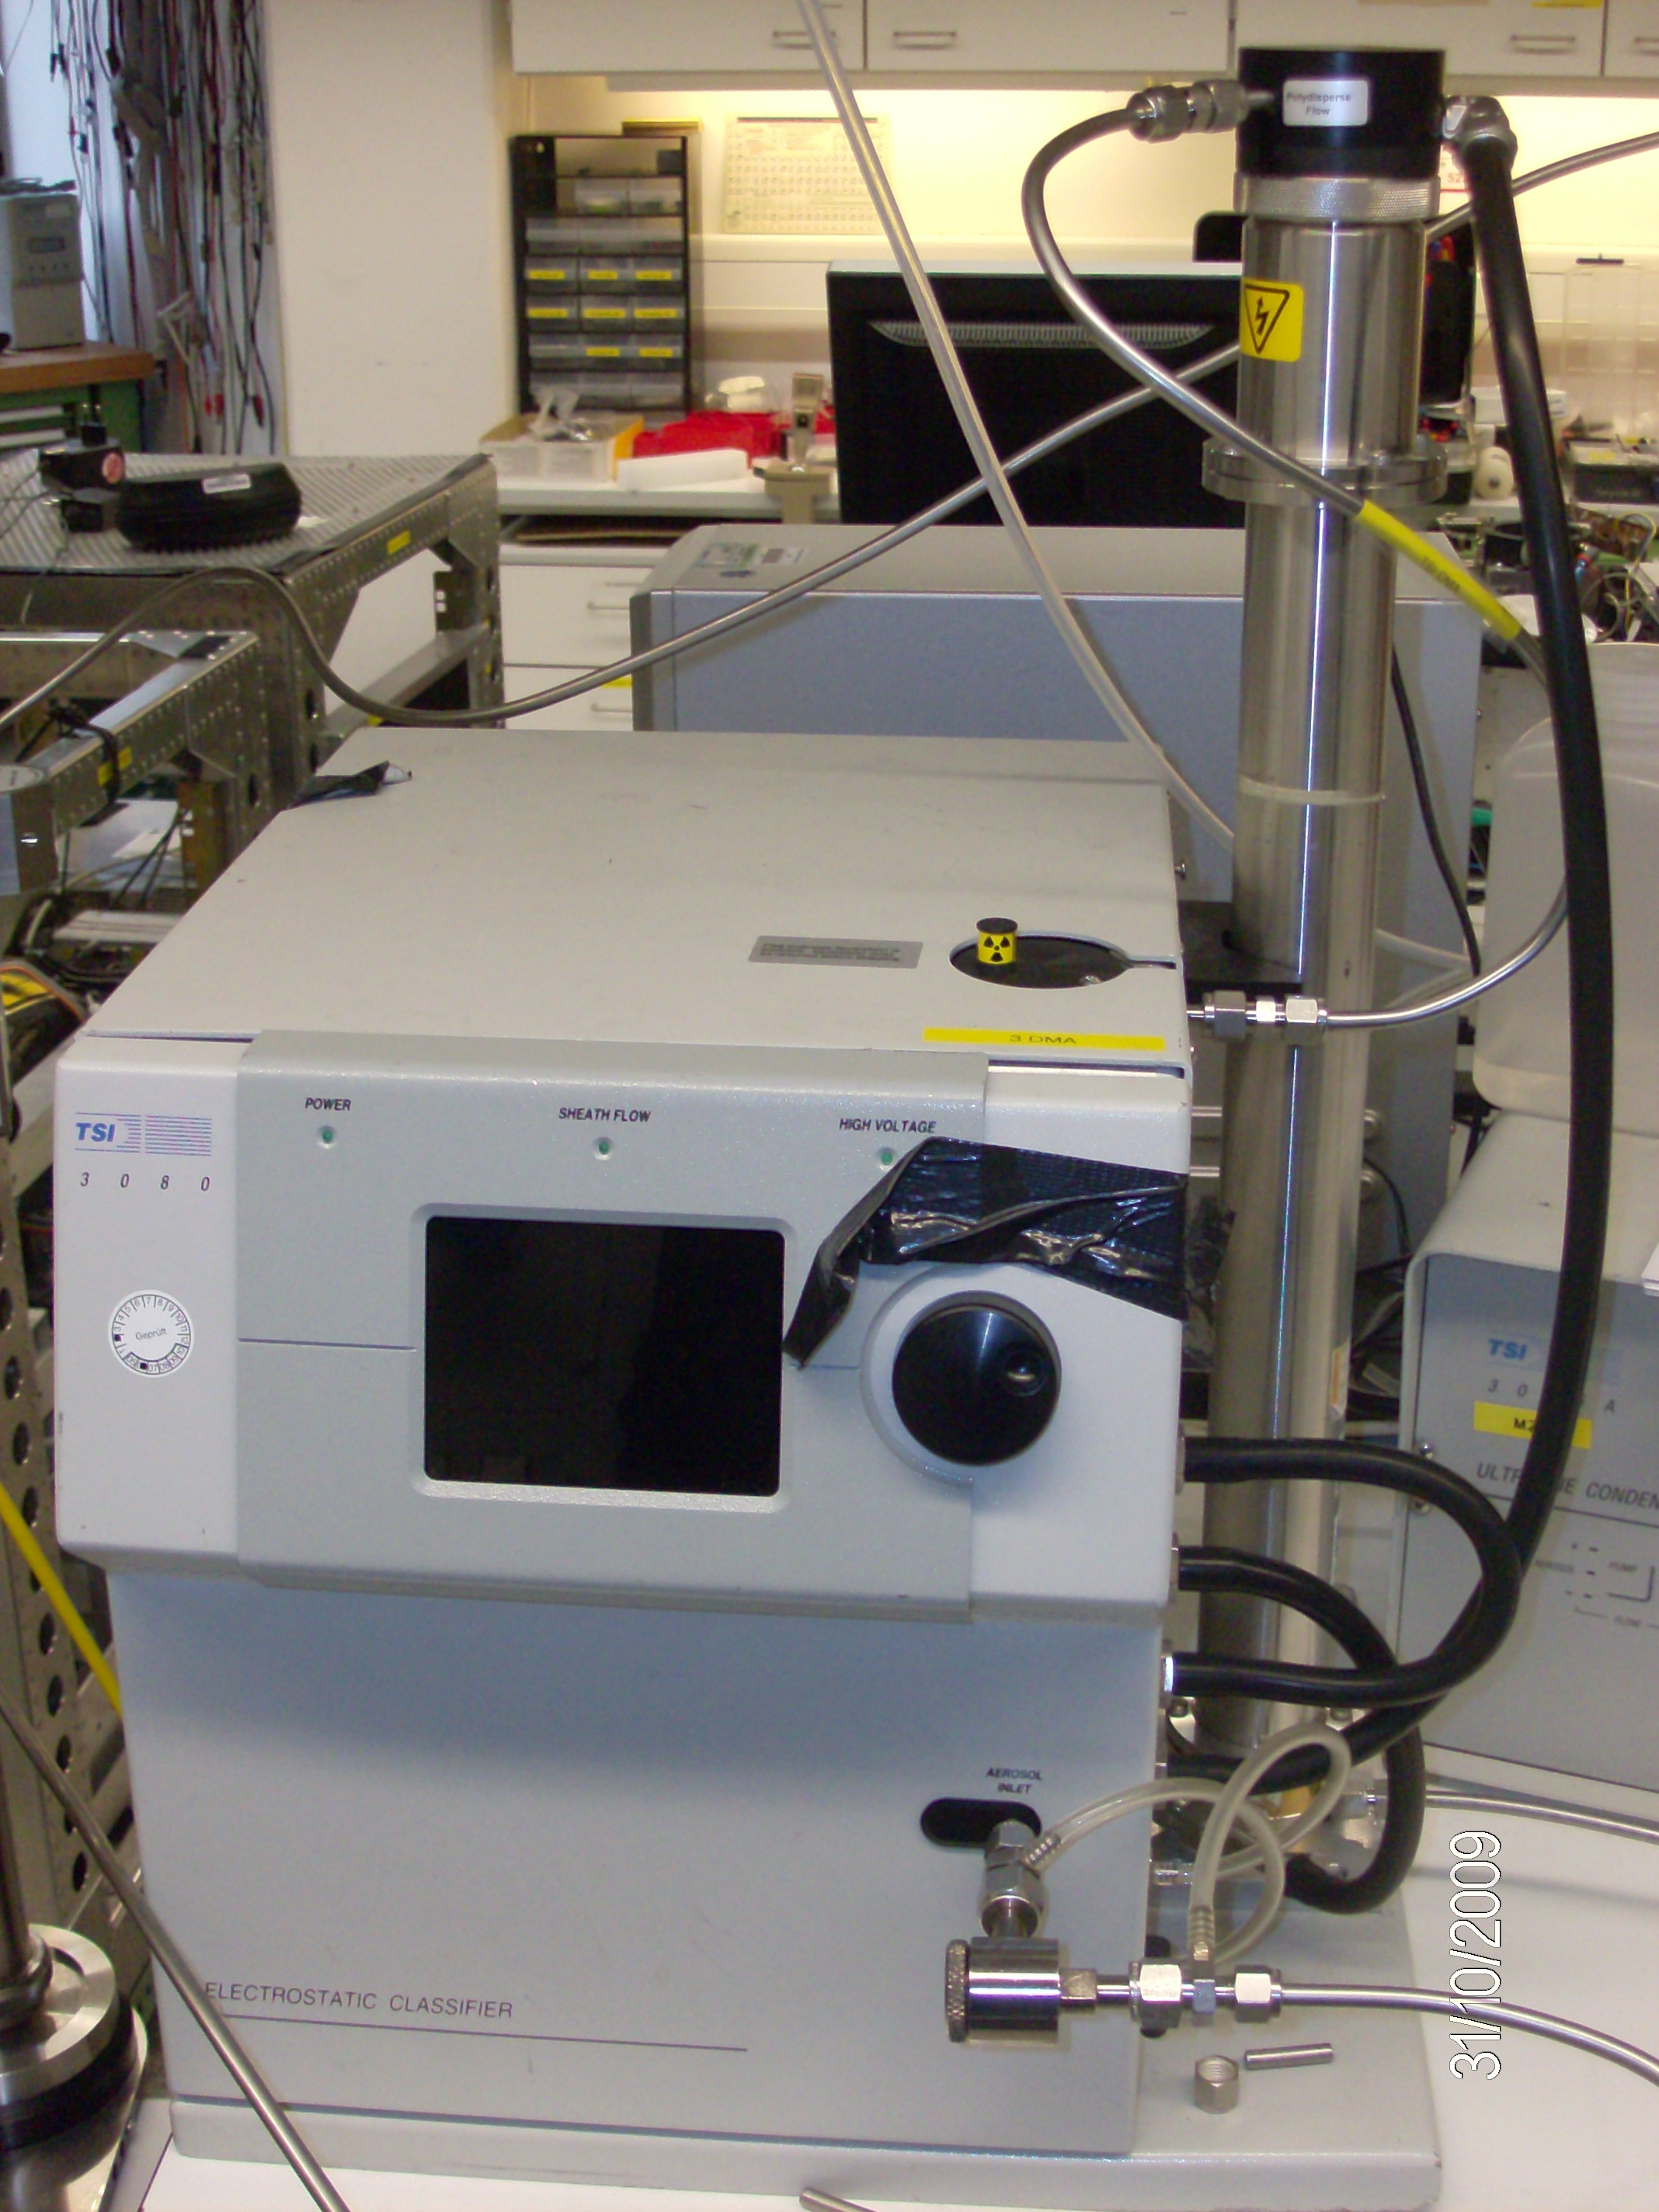
\includegraphics[scale=0.1]{eps/TSI3080CE.eps}\\
\end{center}
\caption{\label{TSI3080CE}\hspace{-0.1em} classificador eletrost\'{a}tico (TSI 3080).}
\end{figure}


\begin{figure}[hbt]
\begin{center}
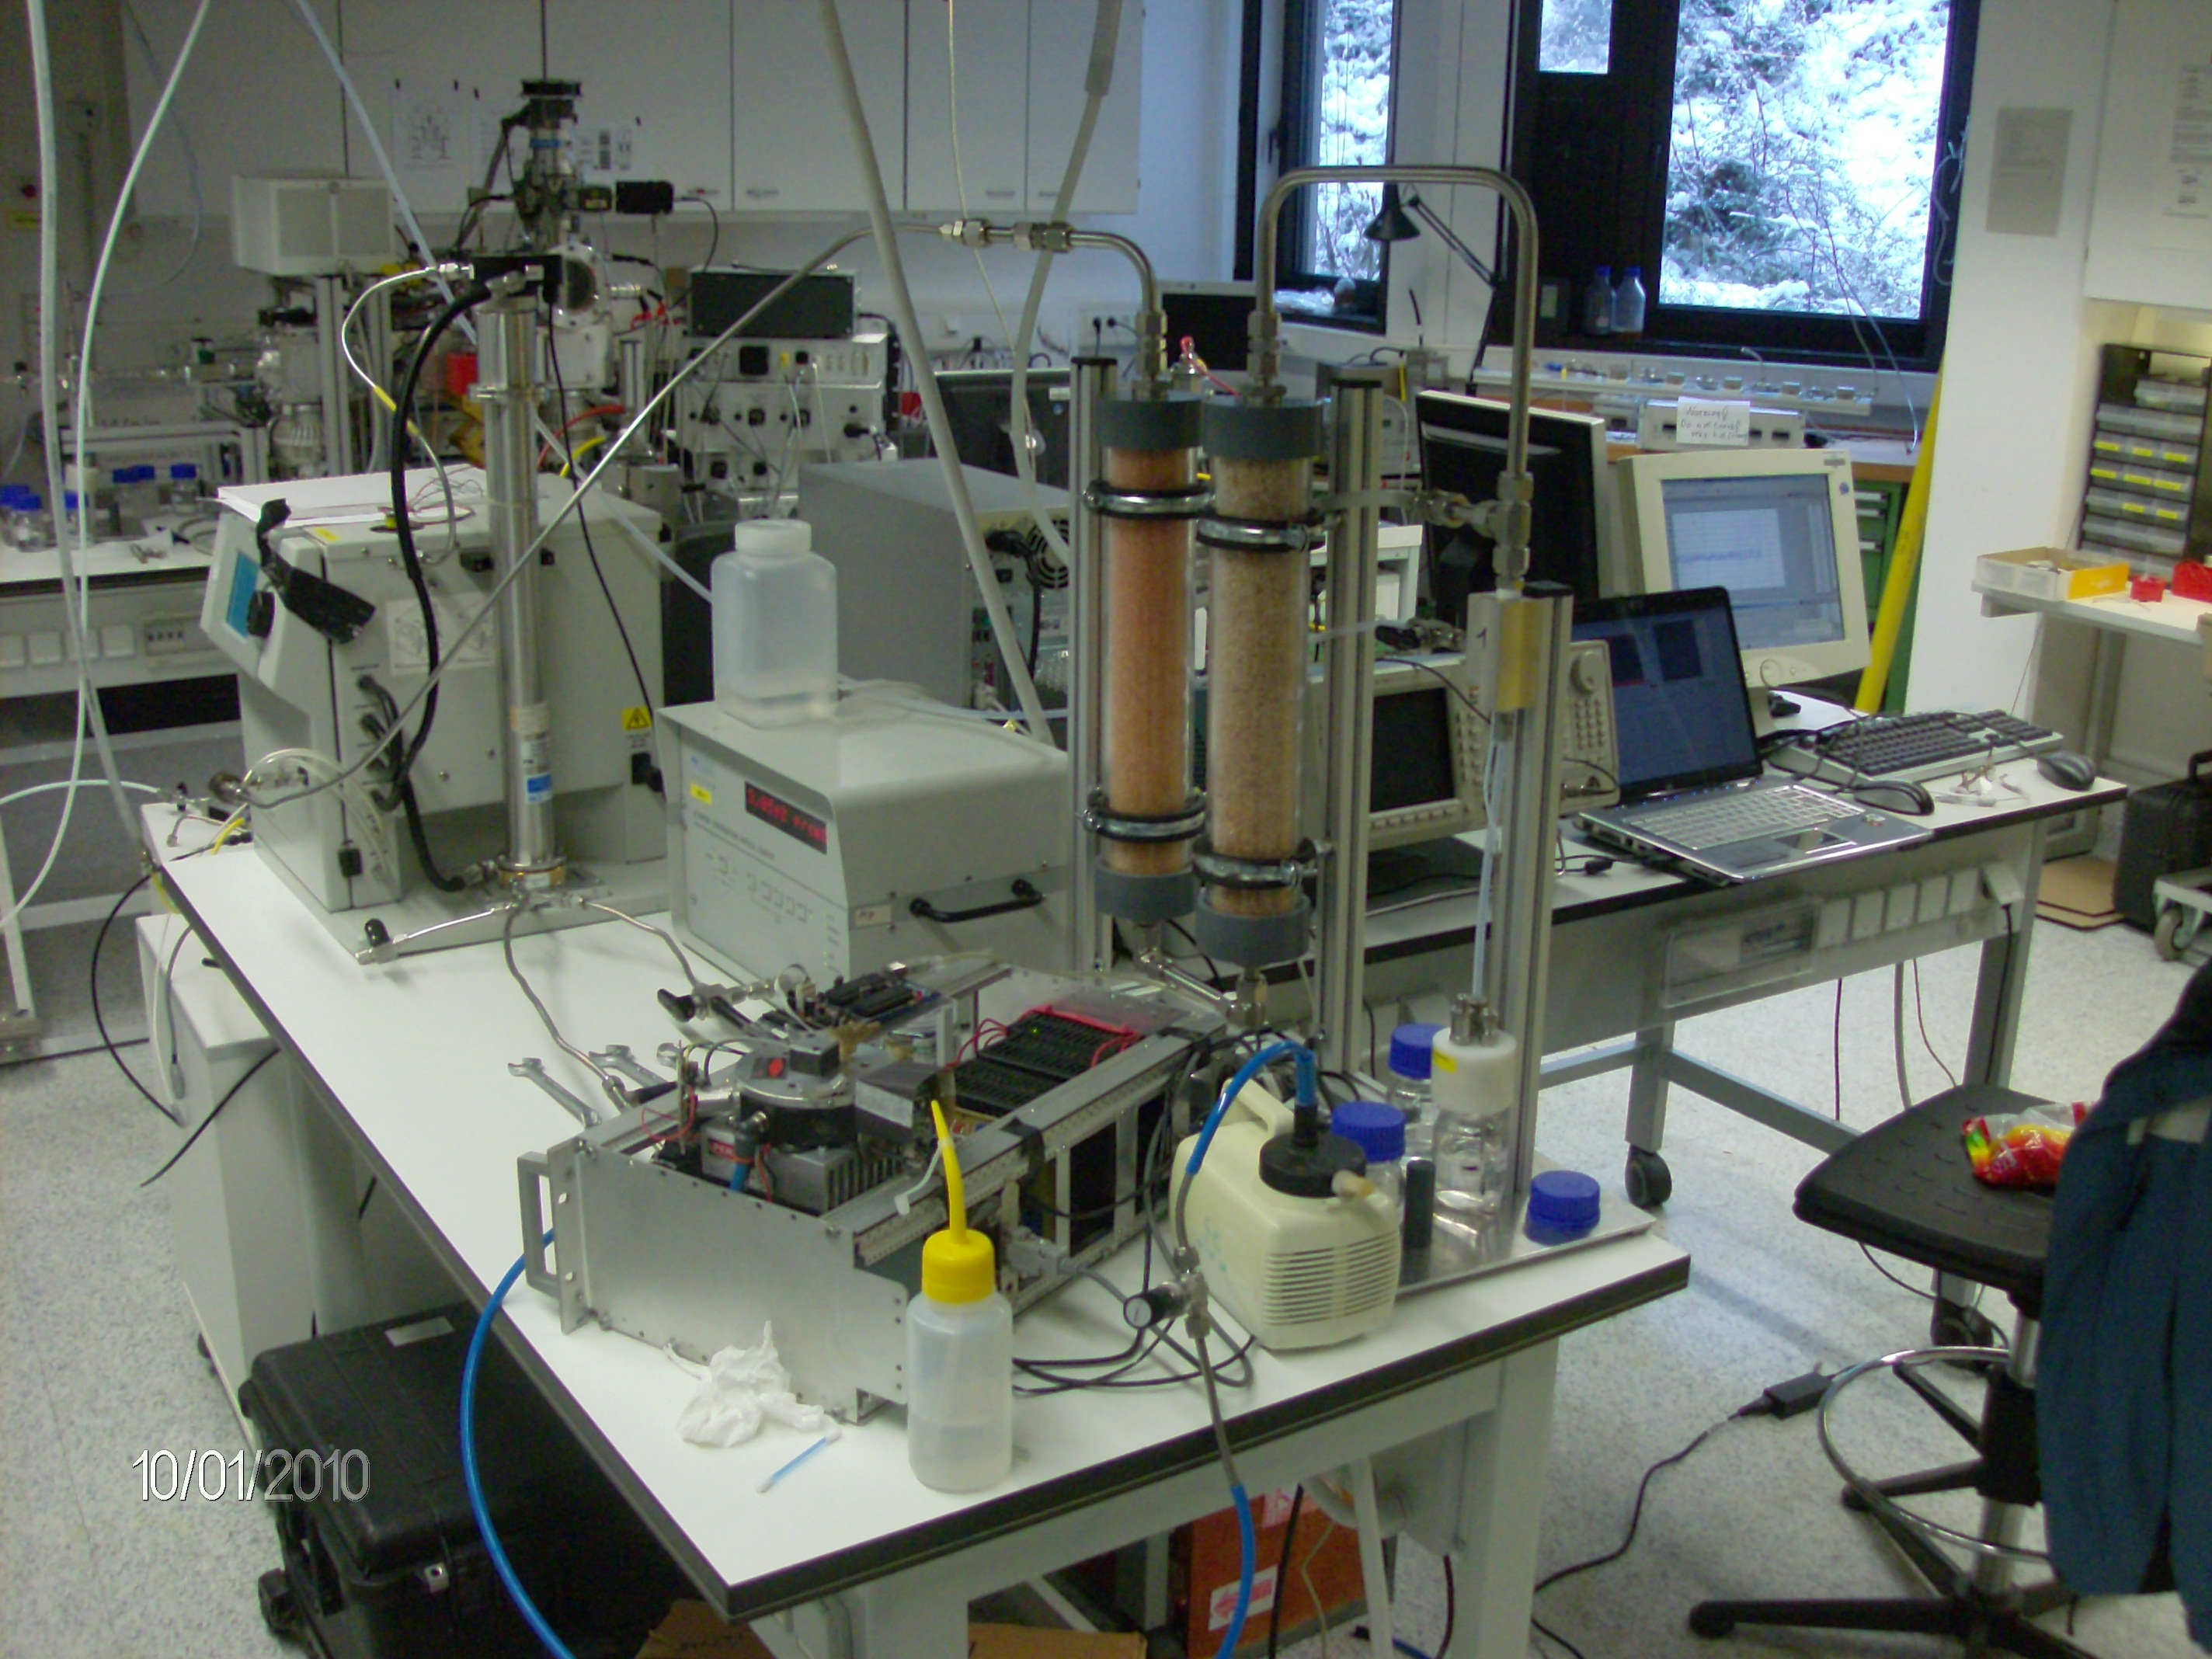
\includegraphics[scale=0.1]{eps/BANCADA_FOTO.eps}\\
\end{center}
\caption{\label{BANCADA_FOTO}\hspace{-0.1em} vista geral da bancada (TSI 3080).}
\end{figure}


\subsection{Prevenindo perda de part\'{\i}culas por deposi\c{c}\~{a}o eletrost\'{a}tica}
As medidas de aeross\'{o}is requerem um sistema de dutos para condu\c{c}\~{a}o destes aeross\'{o}is at\'{e} os mais variados instrumentos de medi\c{c}\~{a}o. Dependendo das caracter\'{\i}sticas f\'{\i}sicas dos aeross\'{o}is e dos dutos, diversos mecanismos de perda de part\'{\i}culas podem interferir nas medi\c{c}\~{o}es \cite{SL}. Uma destas causas chama-se de perda por deposi\c{c}\~{a}o eletrost\'{a}tica. Quando os aeross\'{o}is s\~{a}o produzidos em atomizadores, nebulizadores ou atrav\'{e}s de mecanismos naturais, alguns podem n\~{a}o estar eletricamente neutros. No caso destes aeross\'{o}is serem capturados pelos dutos de qualquer medidor de concentra\c{c}\~{a}o, pode ocorrer de algumas part\'{\i}culas ficarem retinas nos pr\'{o}prios dutos caso estes n\~{a}o sejam de material condutor e n\~{a}o estejam aterrados. Com o objetivo de verificar estas perdas, um experimento foi realizado e consistia em comparar a medida da concentra\c{c}\~{a}o realizada pelo CPC em 2 condi\c{c}\~{o}es: a primeira utilizando um duto coletor de 3 metros de pl\'{a}stico e a segunda utilizando um duto de a\c{c}o inox de mesmo comprimento. A medida foi realizada durante 50 segundos para cada caso. O resultado deste experimento mostrou que este efeito n\~{a}o pode ser negligenciado no caso de dutos longos, pois, a diferen\c{c}a chegou a 13\% na m\'{e}dia como \'{e} mostrado na Tabela \ref{perdas} e na Figura \ref{duto}.


\begin{table}[!htbp]
\centering \caption{\label{perdas} compara\c{c}\~{a}o entre concentra\c{c}\~{o}es medidas realizadas por dutos de a\c{c}o e pl\'{a}stico}
\begin{tabular}{ c | c  }
  \hline
  Tipo de duto & Concentra\c{c}\~{a}o m\'{e}dia\\
  \hline
  A\c{c}o & 2611\\
  Pl\'{a}stico & 2272\\
  \hline
  Diferen\c{c}a & 13 \% \\
  \hline
\end{tabular}\\
\end{table}



\begin{figure}[hbt]
\begin{center}
\includegraphics[scale=1.0]{eps/dutos.eps}\\
\end{center}
\caption{\label{duto}\hspace{-0.1em} perdas em fun\c{c}\~{a}o do tipo de duto. }
\end{figure}





%%%%%%%%%%%%%%%%%%%%%%%%%%%%%%%%%%%%%%%%%%%%%%%%%%%%%%%%%%%%%%%%%
%%%% CAP\'{I}TULO 5: Resultados
\include{ccnc_resultados/ccnc_resultados}
%%%%%%%%%%%%%%%%%%%%%%%%%%%%%%%%%%%%%%%%%%%%%%%%%%%%%%%%%%%%%%%%%
%%%% CAP\'{I}TULO 5.1: Listagem
%%\doublespacing
\documentclass[12pt,a4paper,oneside,final]{book}

\usepackage{listings}
\usepackage{verbatim}

%\usepackage{algorithm}
\usepackage{algorithmic}
%\usepackage{algorithm2e}



\begin{document}

%\begin{algorithm}


\begin{algorithmic}[1]

%\caption{Fast Watershed - Vicent and Soiller}
\STATE{\#define MASK -2}\COMMENT{\textit{coment\'{a}rio}}
\STATE{\#define WSHED 0}
\STATE{\#define INIT -1}
\STATE{entrada: imi /*imagem de entrada*/}
\STATE{sa\'{\i}da: imo /*imagem de sa\'{\i}da*/}
\STATE{ imd /*imagem de trabalho*/}
\STATE{Inicializa\c{c}\~{a}o:}

\STATE{corrent\_label $\leftarrow$ 0}
\STATE{corrent\_dist $\leftarrow$ 0}
%\STATE{$\forall$p $\in$ D$_{imo}$,\ imo(p) $\leftarrow$ INIT}
\STATE{imo $\leftarrow$ INIT}
\STATE{imd$\leftarrow$ 0}
\STATE{Organiza pixels de imi em ordem crescente de n\'{\i}veis de cinza}
\STATE{h$_{min}$ $\leftarrow$ MIN(imi),\ h$_{max}$ $\leftarrow$ MAX(imi)}

\FOR{h=h$_{min}$ to h$_{max}$}
    \FOR{$\forall$p$\mid$ imi(p)=h}
        \STATE{imo(p)$\leftarrow$MASK}
        \IF{$\exists$p'$\in$N$_G$(p)$\mid$ (imo(p')$>$0) ou (imo(p')=WSHED)}
            \STATE{imd(p)$\leftarrow$1}
            \STATE{fifo\_add(p)}
        \ENDIF
    \ENDFOR
    \STATE{current\_dist$\leftarrow$1}
    \STATE{fifo\_add(pixel\_ficticio)}

    \LOOP
        \STATE{p$\leftarrow$fifo\_first()}
        \IF{p=pixel\_ficticio}
            \IF{fifo\_empty()=TRUE}
                \STATE{BREAK}
            \ELSE
                \STATE{fifo\_add(pixel\_ficticio)}
                \STATE{current\_dist $\leftarrow$ current\_dist+1}
                \STATE{p$\leftarrow$fifo\_first()}
            \ENDIF
        \ENDIF
        \FOR{$\forall$p'$\in$N$_G$(p)}
            \IF{imd(p')$<$current\_dist $\ $ and $\ $ (imo(p')$>$0 $\ $ OR imo(p')=WSHED)}

                \IF{imo(p')$>$0}
                    \IF{imo(p)=MASK OR imo(p)=WSHED}
                        \STATE{imo(p)$\leftarrow$imo(p')}
                    \ELSE
                        \IF{imo(p)$\neq$imo(p')}
                            \STATE{imo(p)$\leftarrow$WSHED}
                        \ENDIF
                    \ENDIF
                \ELSE
                    \IF{imo(p)=MASK}
                        \STATE{imo(p)$\leftarrow$WSHED}
                    \ENDIF
                \ENDIF
            \ELSE
                \IF{imo(p')=MASK AND imd(p')=0}
                    \STATE{imd(p')$\leftarrow$current\_dist+1}
                    \STATE{fifo\_add(p')}
                \ENDIF

            \ENDIF
        \ENDFOR
    \ENDLOOP
    \FOR{$\forall$ p $\mid$ imi(p)=h}
        \STATE{imd(p) $\leftarrow$ 0}
        \IF{imo(p)=MASK}
            \STATE{current\_label $\leftarrow$ current\_label+1}
            \STATE{fifo\_add(p)}
            \STATE{imo(p)=current\_label}
            \WHILE {fifo\_empty()=false}
                \STATE{p' $\leftarrow$  fifo\_first()}
                \FOR{$\forall$ p" $\in$ N$_G$(p')}
                    \IF{imo(p")=MASK}
                        \STATE{fifo\_add(p")}
                        \STATE{imo(p")$\leftarrow$current\_label}
                    \ENDIF
                \ENDFOR
            \ENDWHILE
        \ENDIF
    \ENDFOR
           
\ENDFOR
\end{algorithmic}
%\end{algorithm}


\end{document}


%%%%%%%%%%%%%%%%%%%%%%%%%%%%%%%%%%%%%%%%%%%%%%%%%%%%%%%%%%%%%%%%%
%%%% CAP\'{I}TULO 6: Conclus\~{o}es
\doublespacing
%% ------------------------------------------------------------------------- %%

\chapter{Conclus\~{o}es, contribui\c{c}\~{o}es e trabalhos futuros}
\label{cap:conclus\~{o}es}

\PARstartOne{E}{sta} tese prop\~{o}e um novo contador de n\'{u}cleos de condensa\c{c}\~{a}o de nuvens com c\^{a}mara de difus\~{a}o est\'{a}tica, empregando um sistema de vis\~{a}o computacional para a contagem autom\'{a}tica de gotas. Al\'{e}m disso, s\~{a}o descritos e analisados os diversos tipos de CCNCs existentes, apontando-se as principais caracter\'{\i}sticas, bem como suas limita\c{c}\~{o}es. Descreve-se a metodologia de concep\c{c}\~{a}o e desenvolvimento desse novo CCNC, dividindo-se em duas partes: hardware e software.

Quanto \`{a} primeira parte, contempla o esquem\'{a}tico do novo CCNC, o controle de supersatura\c{c}\~{a}o, composto por circuitos el\'{e}tricos projetados especificamente para este fim, contendo um reduzido n\'{u}mero de componentes. A segunda parte, o software, divide-se em dois n\'{u}cleos, sendo o primeiro respons\'{a}vel por permitir a intera\c{c}\~{a}o do novo CCNC com o operador para possibilit\'{a}-lo operar os servi\c{c}os e a configura\c{c}\~{a}o operacional, tais como ajustar o volume de amostragem, o n\'{\i}vel de ilumina\c{c}\~{a}o, entre outros.  O segundo n\'{u}cleo \'{e} composto pelo sistema de vis\~{a}o computacional, composto por um conjunto de algoritmos, que permite a segmenta\c{c}\~{a}o e contagem autom\'{a}tica das gotas, demonstrando-se eficiente mesmo em altas concentra\c{c}\~{o}es em que ocorrem sobreposi\c{c}\~{a}o de gotas. Em equipamentos equivalentes, essa situa\c{c}\~{a}o \'{e} contornada apenas com a utiliza\c{c}\~{a}o de diluidores de gases. Al\'{e}m disso, esse sistema de vis\~{a}o \'{e} respons\'{a}vel pela determina\c{c}\~{a}o autom\'{a}tica do volume de amostragem da c\^{a}mara de nuvens.  A valida\c{c}\~{a}o do novo CCNC \'{e} obtida por compara\c{c}\~{a}o com um CPC, produzindo-se concentra\c{c}\~{o}es de aeross\'{o}is neste e comparando-se com as concentra\c{c}\~{o}es medidas pelo novo CCNC, resultando numa correla\c{c}\~{a}o de 99\% entre as medidas.

Com base nos resultados experimentais conclui-se que o novo CCNC pode ser empregado na medi\c{c}\~{a}o de CCNs, inclusive em situa\c{c}\~{o}es de atmosferas polu\'{\i}das, onde h\'{a} alta concentra\c{c}\~{a}o de aeross\'{o}is. Conclui-se tamb\'{e}m que esse CCNC, por possuir baixos peso e consumo de energia e pode ser embarcado mais facilmente em aeronaves menores.
	
A expans\~{a}o da capacidade de contagem de gotas para cerca de 4000 part\'{\i}culas/cm$^3$, sem o emprego de diluidores de gases e bem acima de outros CCNCs como, por exemplo, o CCNC-MPIChemie (CCNC do Instituto Max Plank para Qu\'{\i}mica da Universidade de Mainz-Alemanha), constitui uma contribui\c{c}\~{a}o importante, pois, permite a medi\c{c}\~{a}o de CCNs em muitas situa\c{c}\~{o}es que atualmente s\~{a}o de interesse cient\'{\i}fico como no caso de atmosferas polu\'{\i}das.
	
Uma nova metodologia para determina\c{c}\~{a}o do valor do volume de amostragem tamb\'{e}m \'{e} apresentada, sendo que essa garante medidas confi\'{a}veis dentro de uma ampla faixa de concentra\c{c}\~{a}o de n\'{u}cleos  de condensa\c{c}\~{a}o de nuvens e dispensa necessidade de uma calibra\c{c}\~{a}o em bancada.
	
Al\'{e}m das contribui\c{c}\~{o}es mencionadas, destacam-se tamb\'{e}m que todo o material usado no projeto do novo CCNC \'{e} facilmente encontrado no mercado nacional e a intensiva utiliza\c{c}\~{a}o de tecnologia digital permitiu a constru\c{c}\~{a}o de um prot\'{o}tipo de baixo peso, de baixo consumo de energia e de pequeno volume se comparado com outros contadores equivalentes.

Como sugest\~{a}o de trabalhos futuros, visando o aperfei\c{c}oamento do novo CCNC, podem-se relacionar:

1.	substituir o a fonte de luz LASER a g\'{a}s (HeNe) por outra fonte de luz LASER baseada em semicondutor. Pode-se citar tr\^{e}s bons motivos: redu\c{c}\~{a}o de peso, de consumo de energia e de custo do CCNC-SDCC. Do ponto de vista mec\^{a}nico este \'{e} um procedimento simples porque a c\^{a}mara de nuvens foi constru\'{\i}da com acess\'{o}rios prevendo essa possibilidade. Entretanto no que diz respeito a metodologia de determina\c{c}\~{a}o do volume de amostragem, essa dever\'{a} sofrer adapta\c{c}\~{o}es pois normalmente a geometria do feixe do LASER semicondutor n\~{a}o \'{e} perfeitamente cil\'{\i}ndrico;

2.	embarcar o sistema de vis\~{a}o computacional e de interface homem m\'{a}quina no \emph{hardware} do pr\'{o}prio CCNC-SDCC. Isto feito, dispensa a utiliza\c{c}\~{a}o de um computador para tal. Nesse sentido, passos j\'{a} foram dados, pois, o c\'{o}digo de processamento de imagem foi implementado em linguagem de program\c{c}\~{a}o C-ANSI;

3.	colocar outra c\^{a}mera digital numa janela da c\^{a}mara para permitir uma vis\~{a}o tridimensional das gotas, podendo ser rastreado o processo de crescimento, inclusive, extraindo-se medidas;

4.	dispor o CCNC de um sistema elet\^{o}nico que permita a transmiss\~{a}o dos dados por GPRS, facilitando o embarque deste equipamento em microaeronaves n\~{a}o tripuladas;

5. disponibilizar o histograma de tamanho de got\'{\i}culas. Isto \'{e} totalmente fact\'{\i}vel a partir da substitui\c{c}\~{a}o da atual \emph{webcam} por outra de alta defini\c{c}\~{a}o de modo a permitir uma melhor rela\c{c}\~{a}o  \emph{pixels}/milimetros.

%%%%%%%%%%%%%%%%%%%%%%%%%%%%%%%%%%%%%%%%%%%%%%%%%%%%%%%%%%%%%%%%%
%%% AP\^{E}NDICE
%\appendix
\begin{appendices}
    \include{ccnc_aerossois/ccnc_aerossois}
    \doublespacing
%% ------------------------------------------------------------------------- %%
\chapter{Bancada geradora de Aeross\'{o}is}
\label{cap:bancada}

O processo de gera\c{c}\~{a}o de aeross\'{o}is inicia-se em um compressor com sa\'{\i}da de ar filtrado. Em seguida, este ar filtrado passa por uma armadilha de \'{a}gua. Nesse ponto, o ar pressurizado, filtrado e seco \'{e} injetado no atomizador TSI3076 que esta acoplado a um reservat\'{o}rio, contendo uma solu\c{c}\~{a}o de sulfato de am\^{o}nia (NH$_4$)$_2$SO$_4$. Outras subst\^{a}ncias higrosc\'{o}picas podem ser utilizadas como por exemplo nitrato de am\^{o}nia NH$_4$NO$_3$, cloreto de s\'{o}dio NaCl e etc. Na sa\'{\i}da deste atomizador, tem-se os aeross\'{o}is propriamente dito, embora polidisperssivo e com uma umidade muito alta. A remo\c{c}\~{a}o da umidade \'{e} feita por um secador a base de silicagel.

Como o processo de condensa\c{c}\~{a}o do vapor de \'{a}gua \'{e} altamente dependente do tamanho do aerossol, ou seja , do tamanho do n\'{u}cleo de condensa\c{c}\~{a}o, exige-se um controle deste par\^{a}metro. Isto \'{e}, exige-se que o aerossol seja monodispersivo. Para tal, utiliza-se na sa\'{\i}da do secador um classificador eletrost\'{a}tico, que no caso \'{e} o TSI3080. Por fim, a medida da concentra\c{c}\~{a}o das part\'{\i}culas \'{e} feita por um contador de part\'{\i}culas condens\'{a}veis (CPC), no caso o TSI3025A.

O contador de part\'{\i}culas condens\'{a}veis  TSI3025A \'{e} capaz de medir aeross\'{o}is com um di\^{a}metro de 3nm at\'{e} 3$\mu$m numa faixa de concentra\c{c}\~{a}o  de 0 at\'{e} 9,99$\cdot$10$^{4}$ part\'{\i}culas / cm$^{3}$. Em condi\c{c}\~{o}es normais, seu sensor de part\'{\i}culas opera em uma atmosfera saturada de Butanol-1.  Essa caracter\'{\i}stica o torna sens\'{\i}vel,  n\~{a}o apenas aos aeross\'{o}is respons\'{a}veis pela forma\c{c}\~{a}o das nuvens e das chuvas, mas a qualquer aerossol. Por essa raz\~{a}o, no processo de compara\c{c}\~{a}o, normalmente se utiliza apenas aeross\'{o}is higrosc\'{o}picos (como por exemplo o sulfato de am\^{o}nia, nitrato de am\^{o}nia ou cloreto de s\'{o}dio) que s\~{a}o capazes de sensibilizar tanto o CCNC-SDCC quanto o CPC TSI3025A.


\begin{figure}[hbt]
\begin{center}
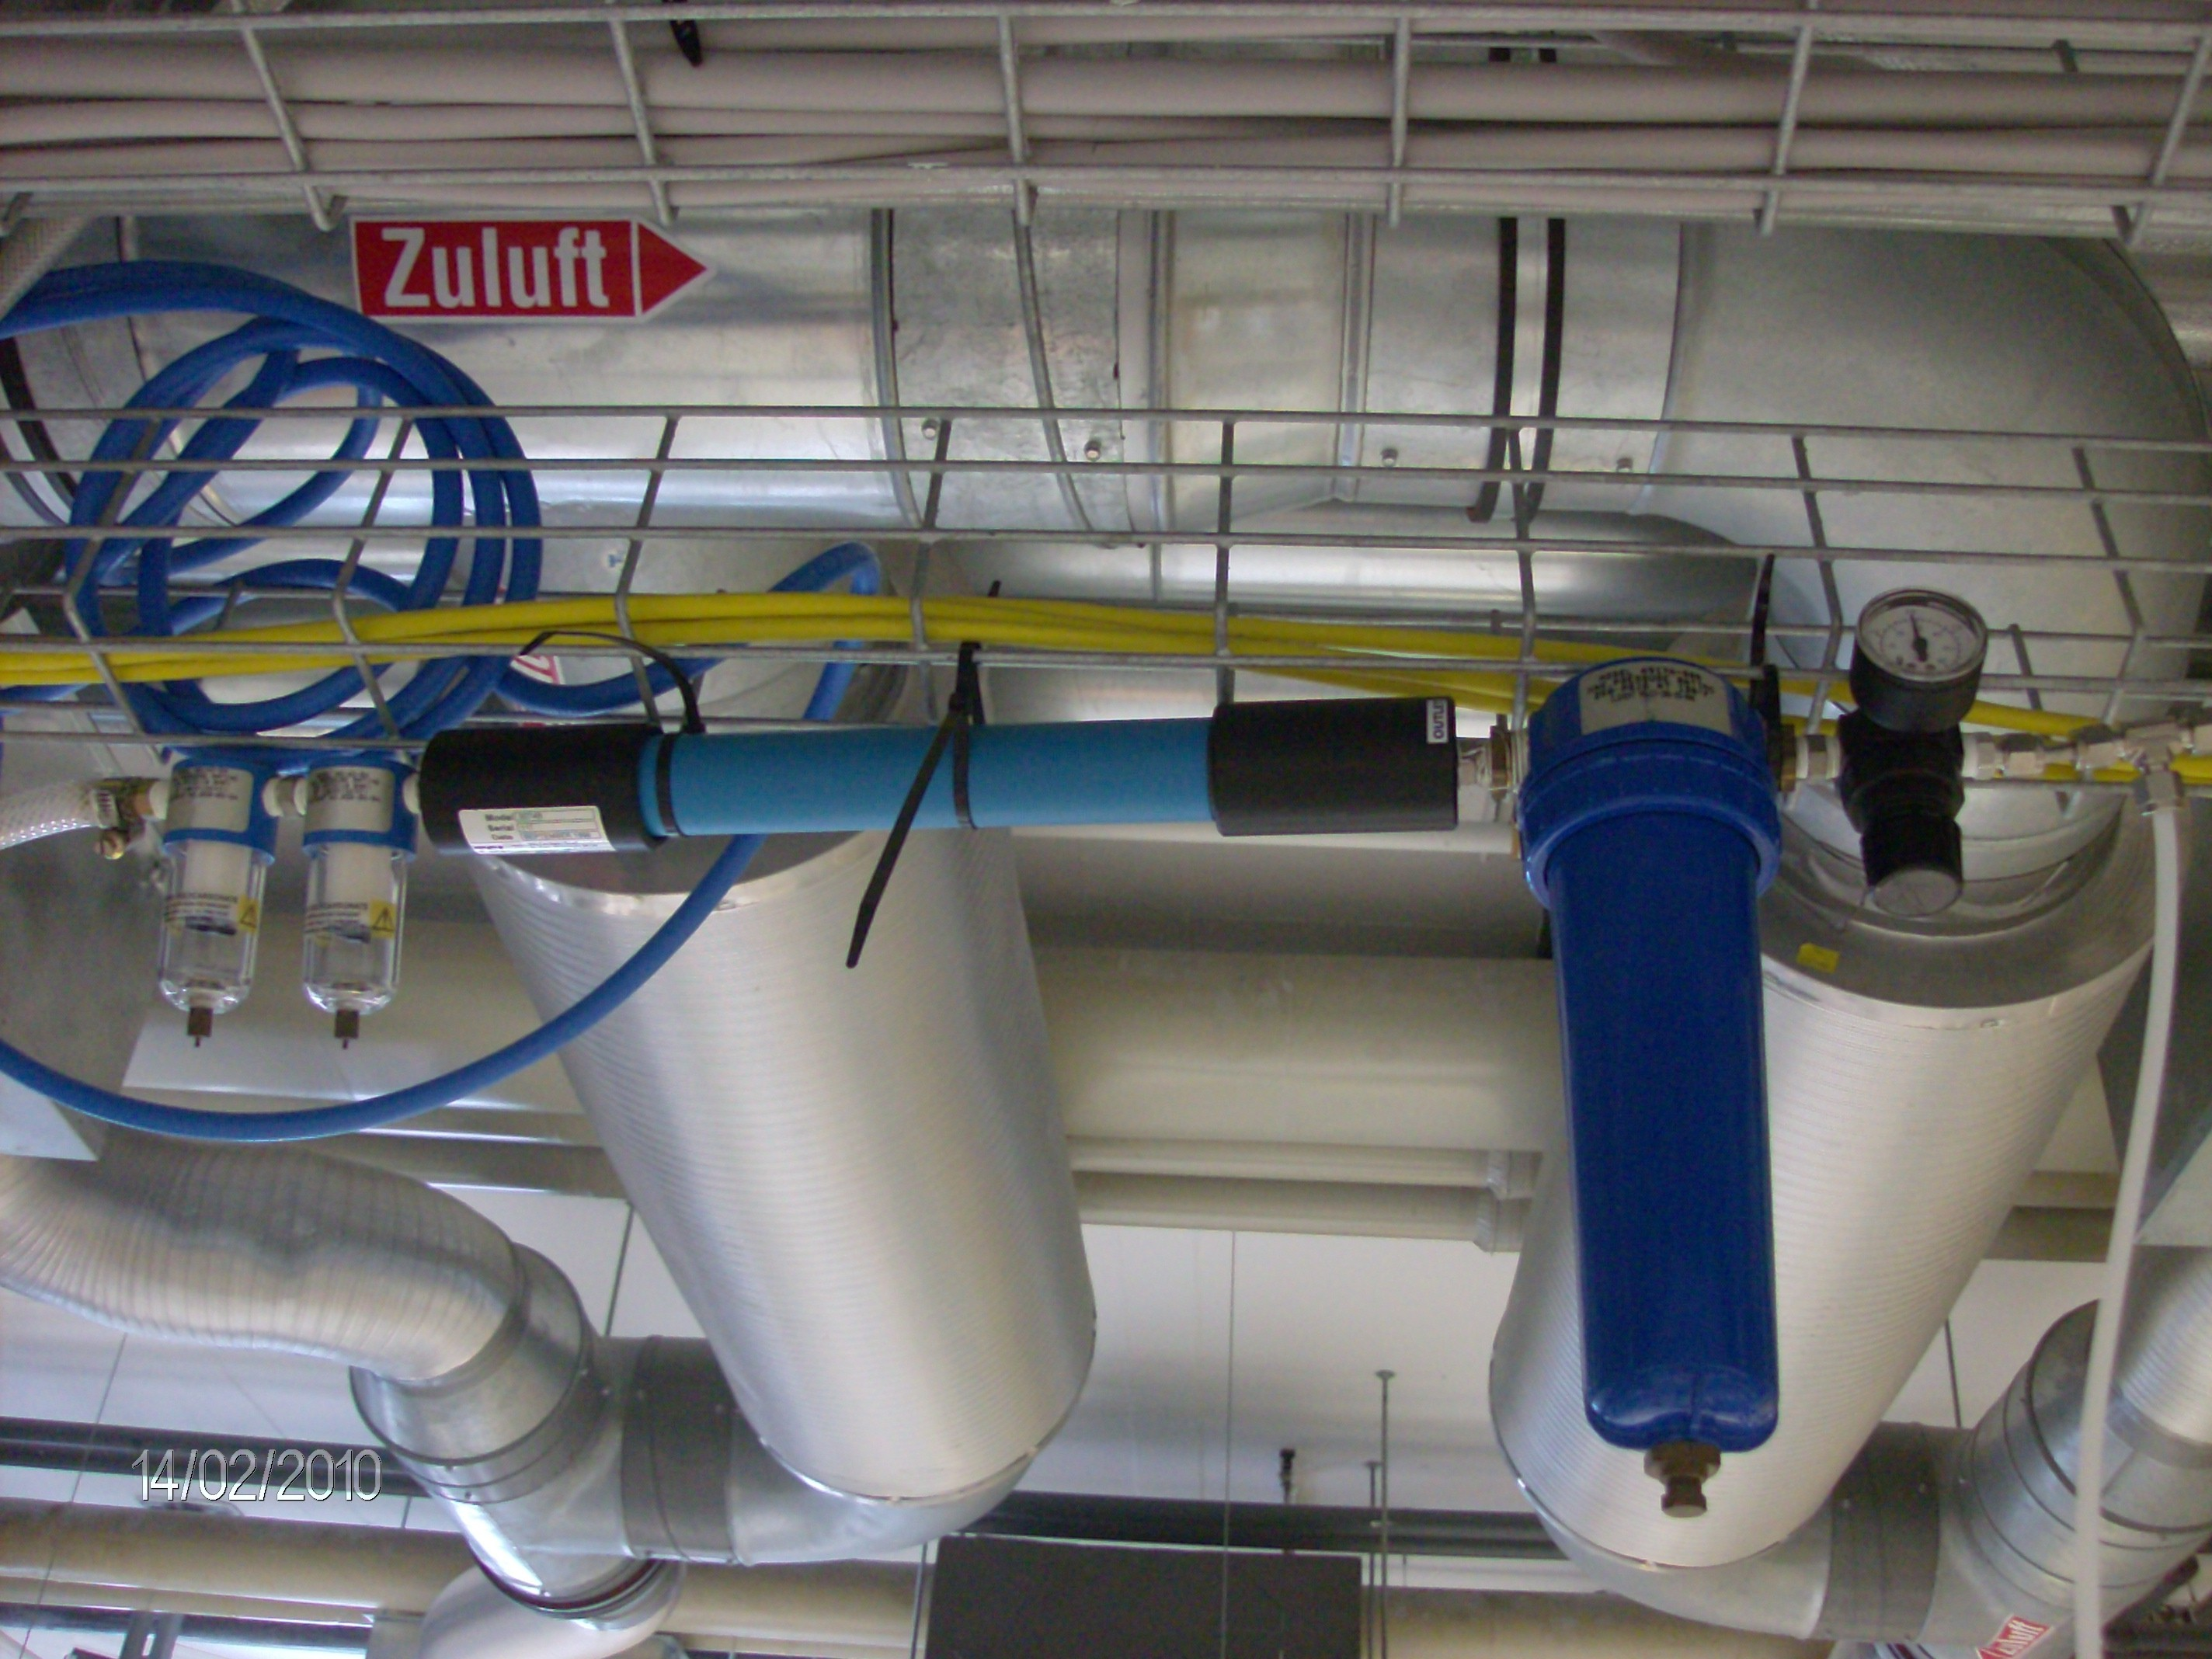
\includegraphics[scale=0.1]{eps/TSI3074FILTRO.eps}\\
\end{center}
\caption{\label{TSI3074FILTRO}\hspace{-0.1em} filtro para remo\c{c}\~{a}o de gotas de \'{o}leo, \'{a}gua e particulados (TSI3074B). }
\end{figure}

\begin{figure}[hbt]
\begin{center}
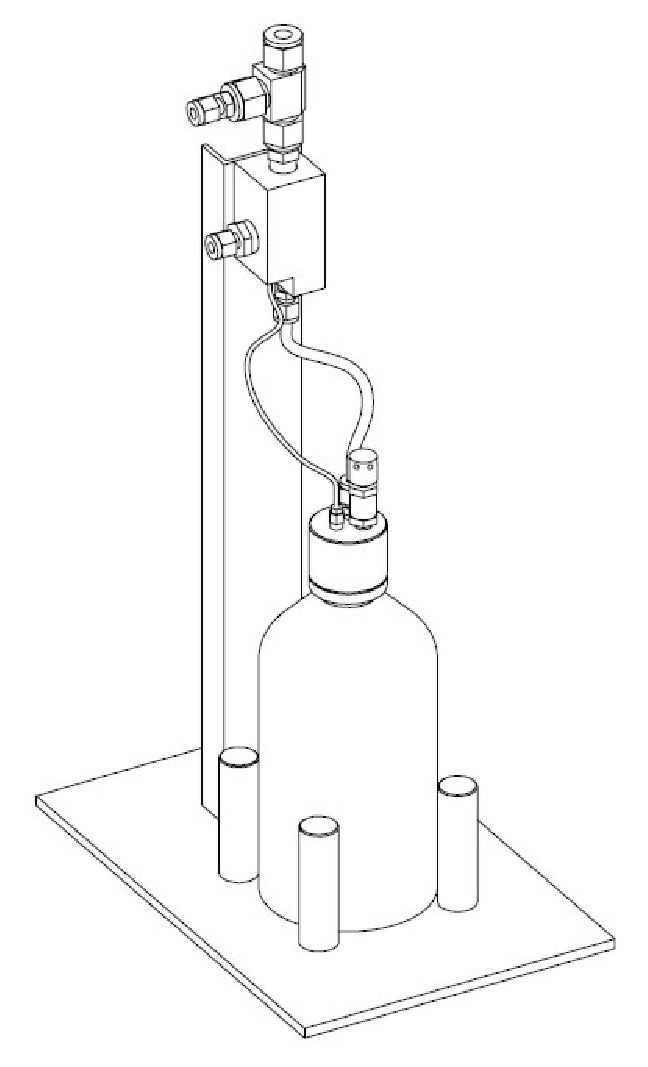
\includegraphics[scale=0.5]{eps/TSI3076ATOMIZADOR.eps}\\
\end{center}
\caption{\label{TSI3074FILTRO}\hspace{-0.1em} diagrama esquem\'{a}tico do atomizador (TSI3076).}
\end{figure}

\begin{figure}[hbt]
\begin{center}
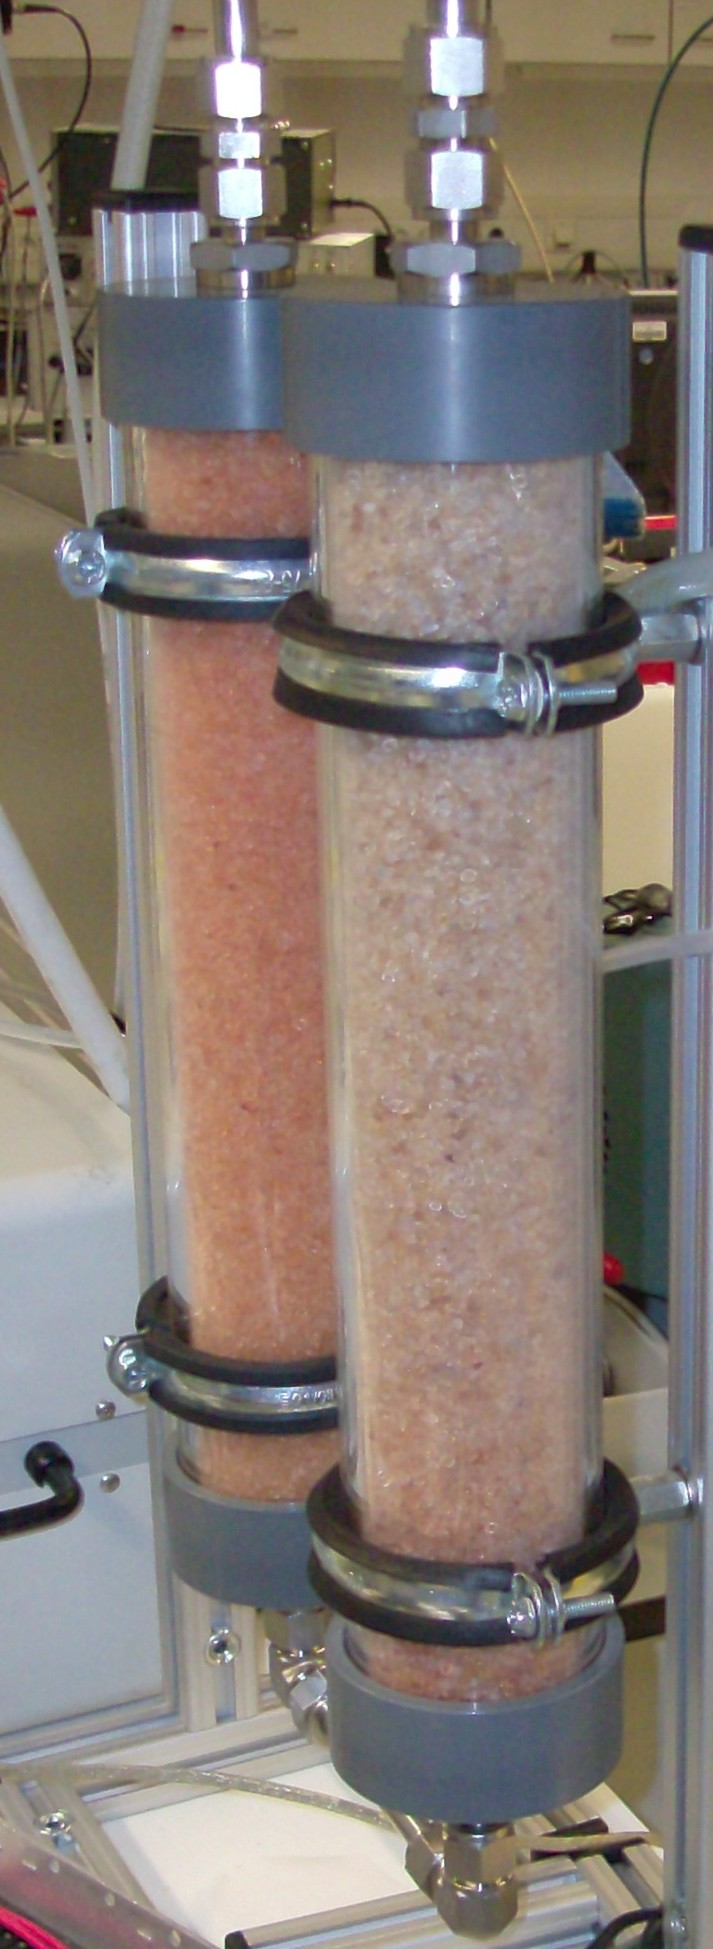
\includegraphics[scale=0.1]{eps/TSI3062SECADOR.eps}\\
\end{center}
\caption{\label{TSI3062SECADOR}\hspace{-0.1em} secador (TSI3062).}
\end{figure}



\begin{figure}[hbt]
\begin{center}
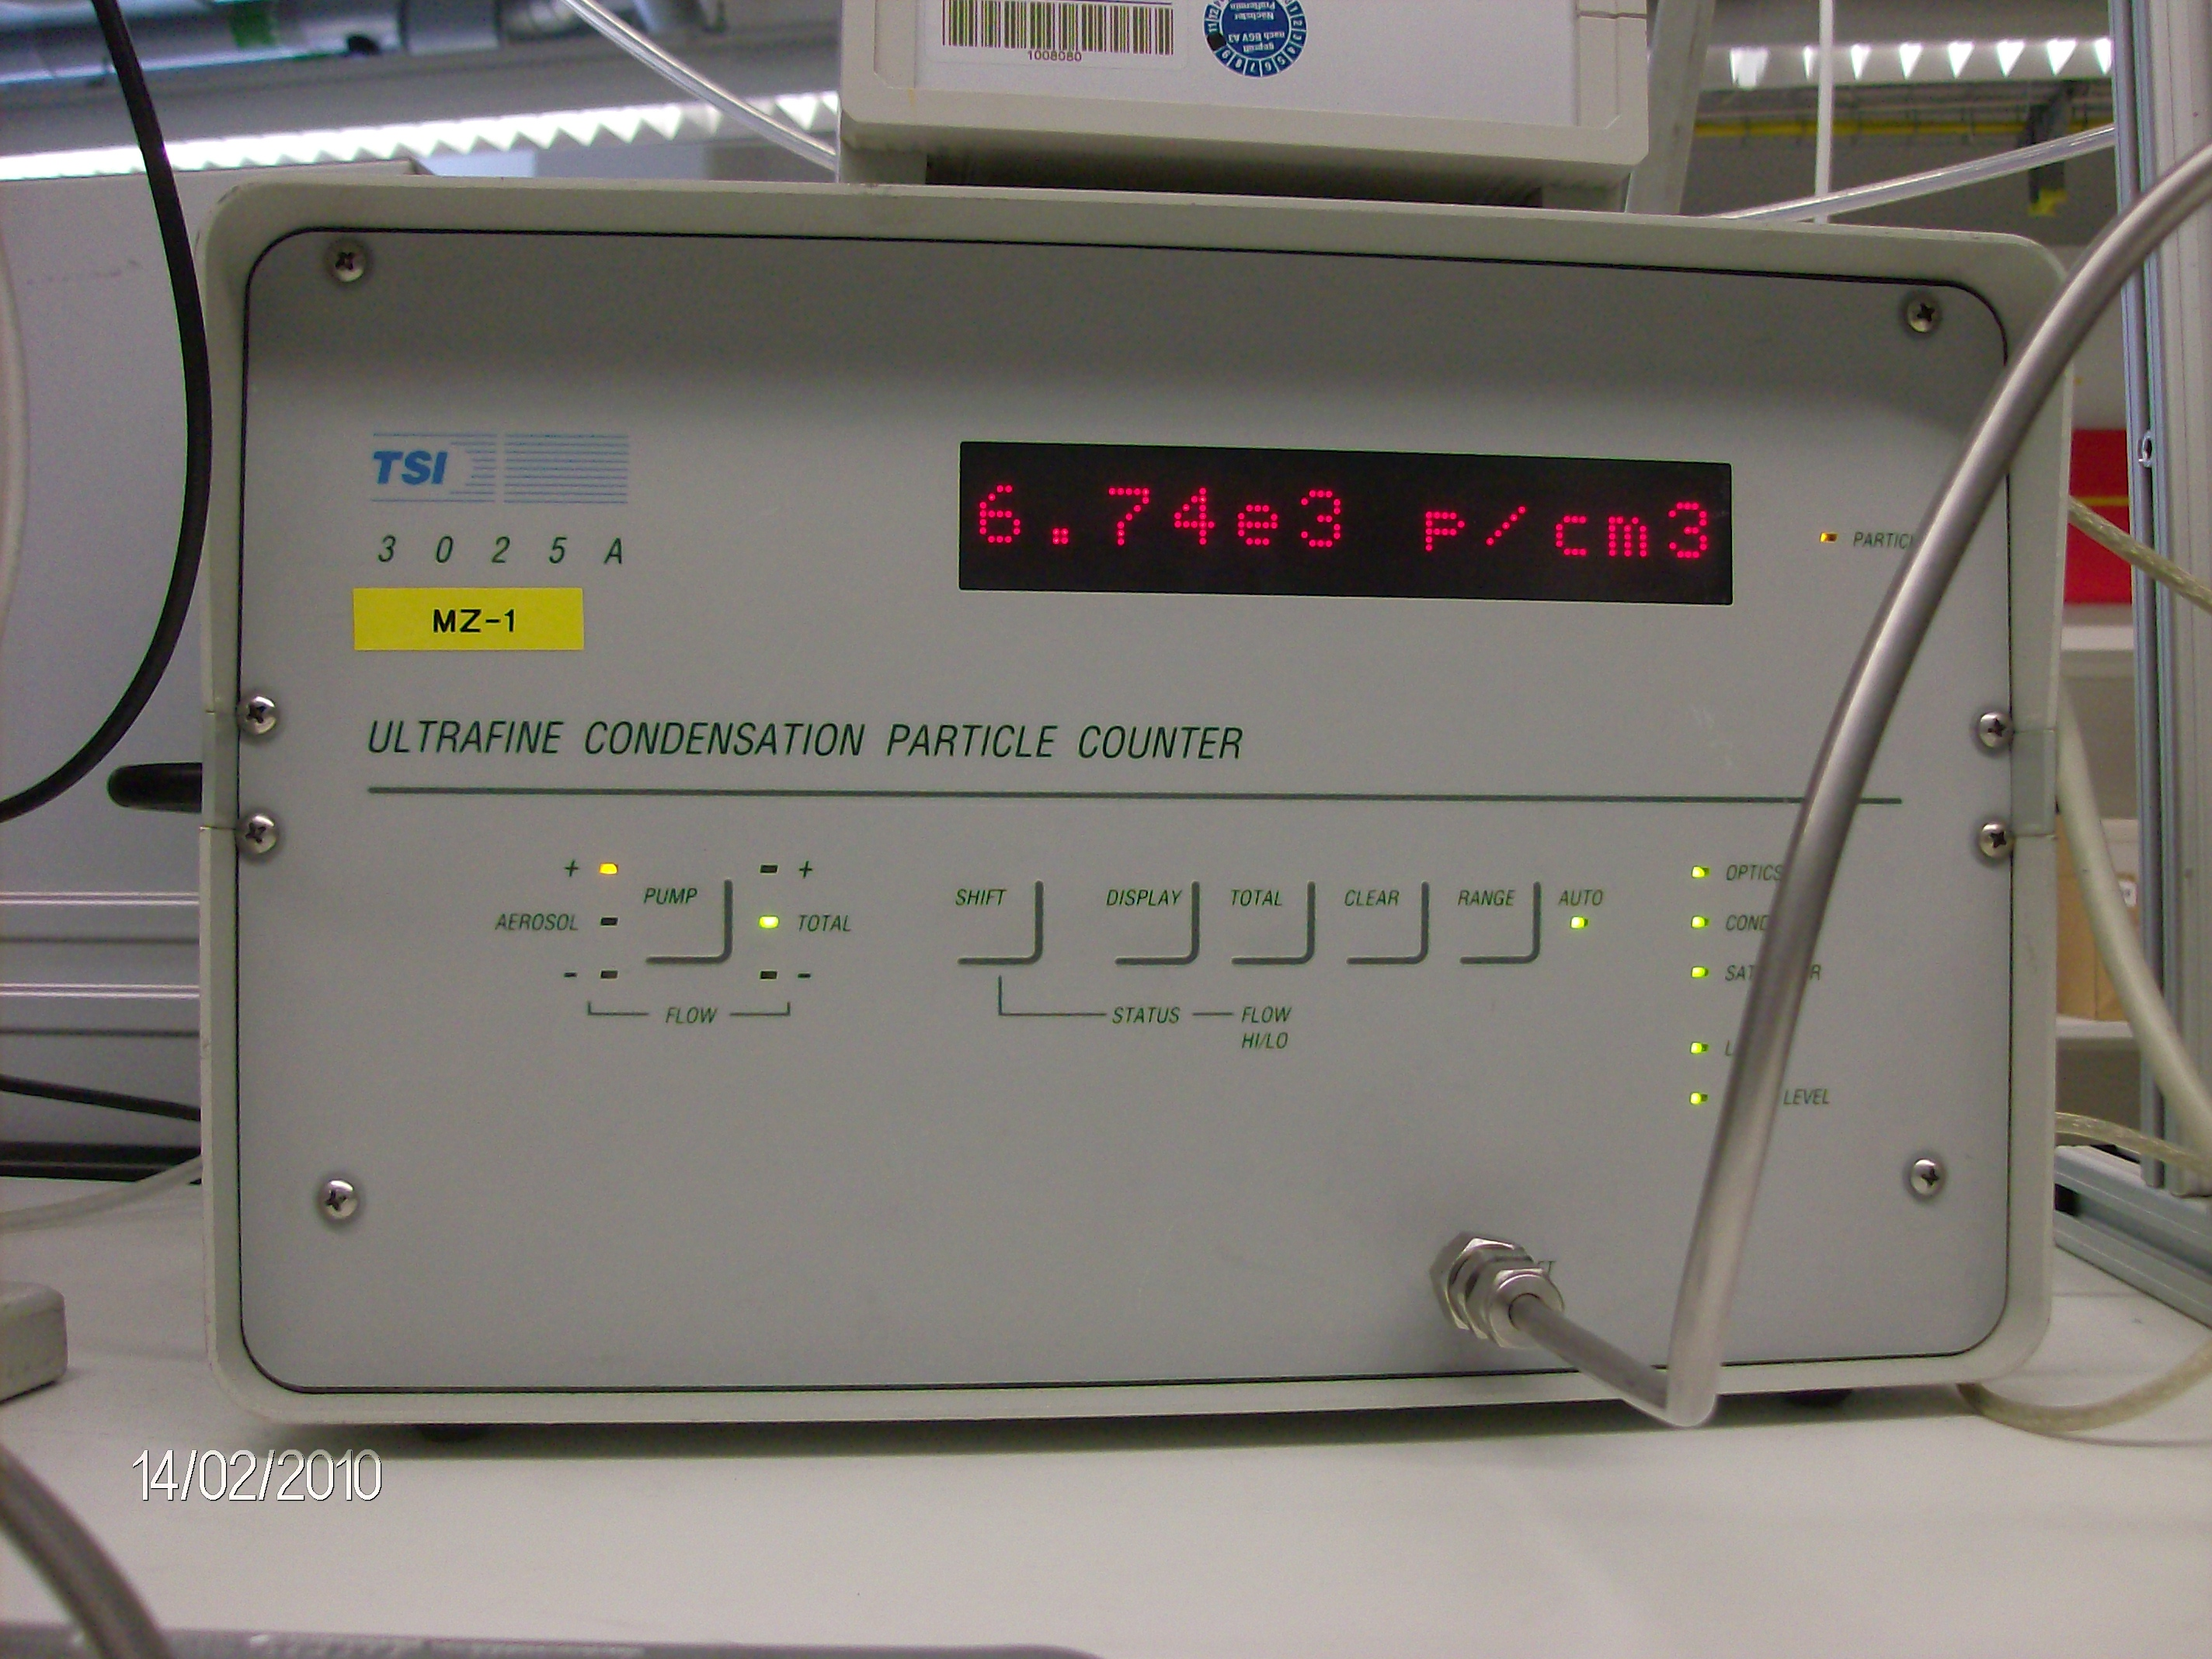
\includegraphics[scale=0.9]{eps/TSI3025CPC.eps}\\
\end{center}
\caption{\label{TSI3025CPC}\hspace{-0.1em} contador de part\'{\i}culas condens\'{a}veis  CPC (TSI 3025A).}
\end{figure}

\begin{figure}[hbt]
\begin{center}
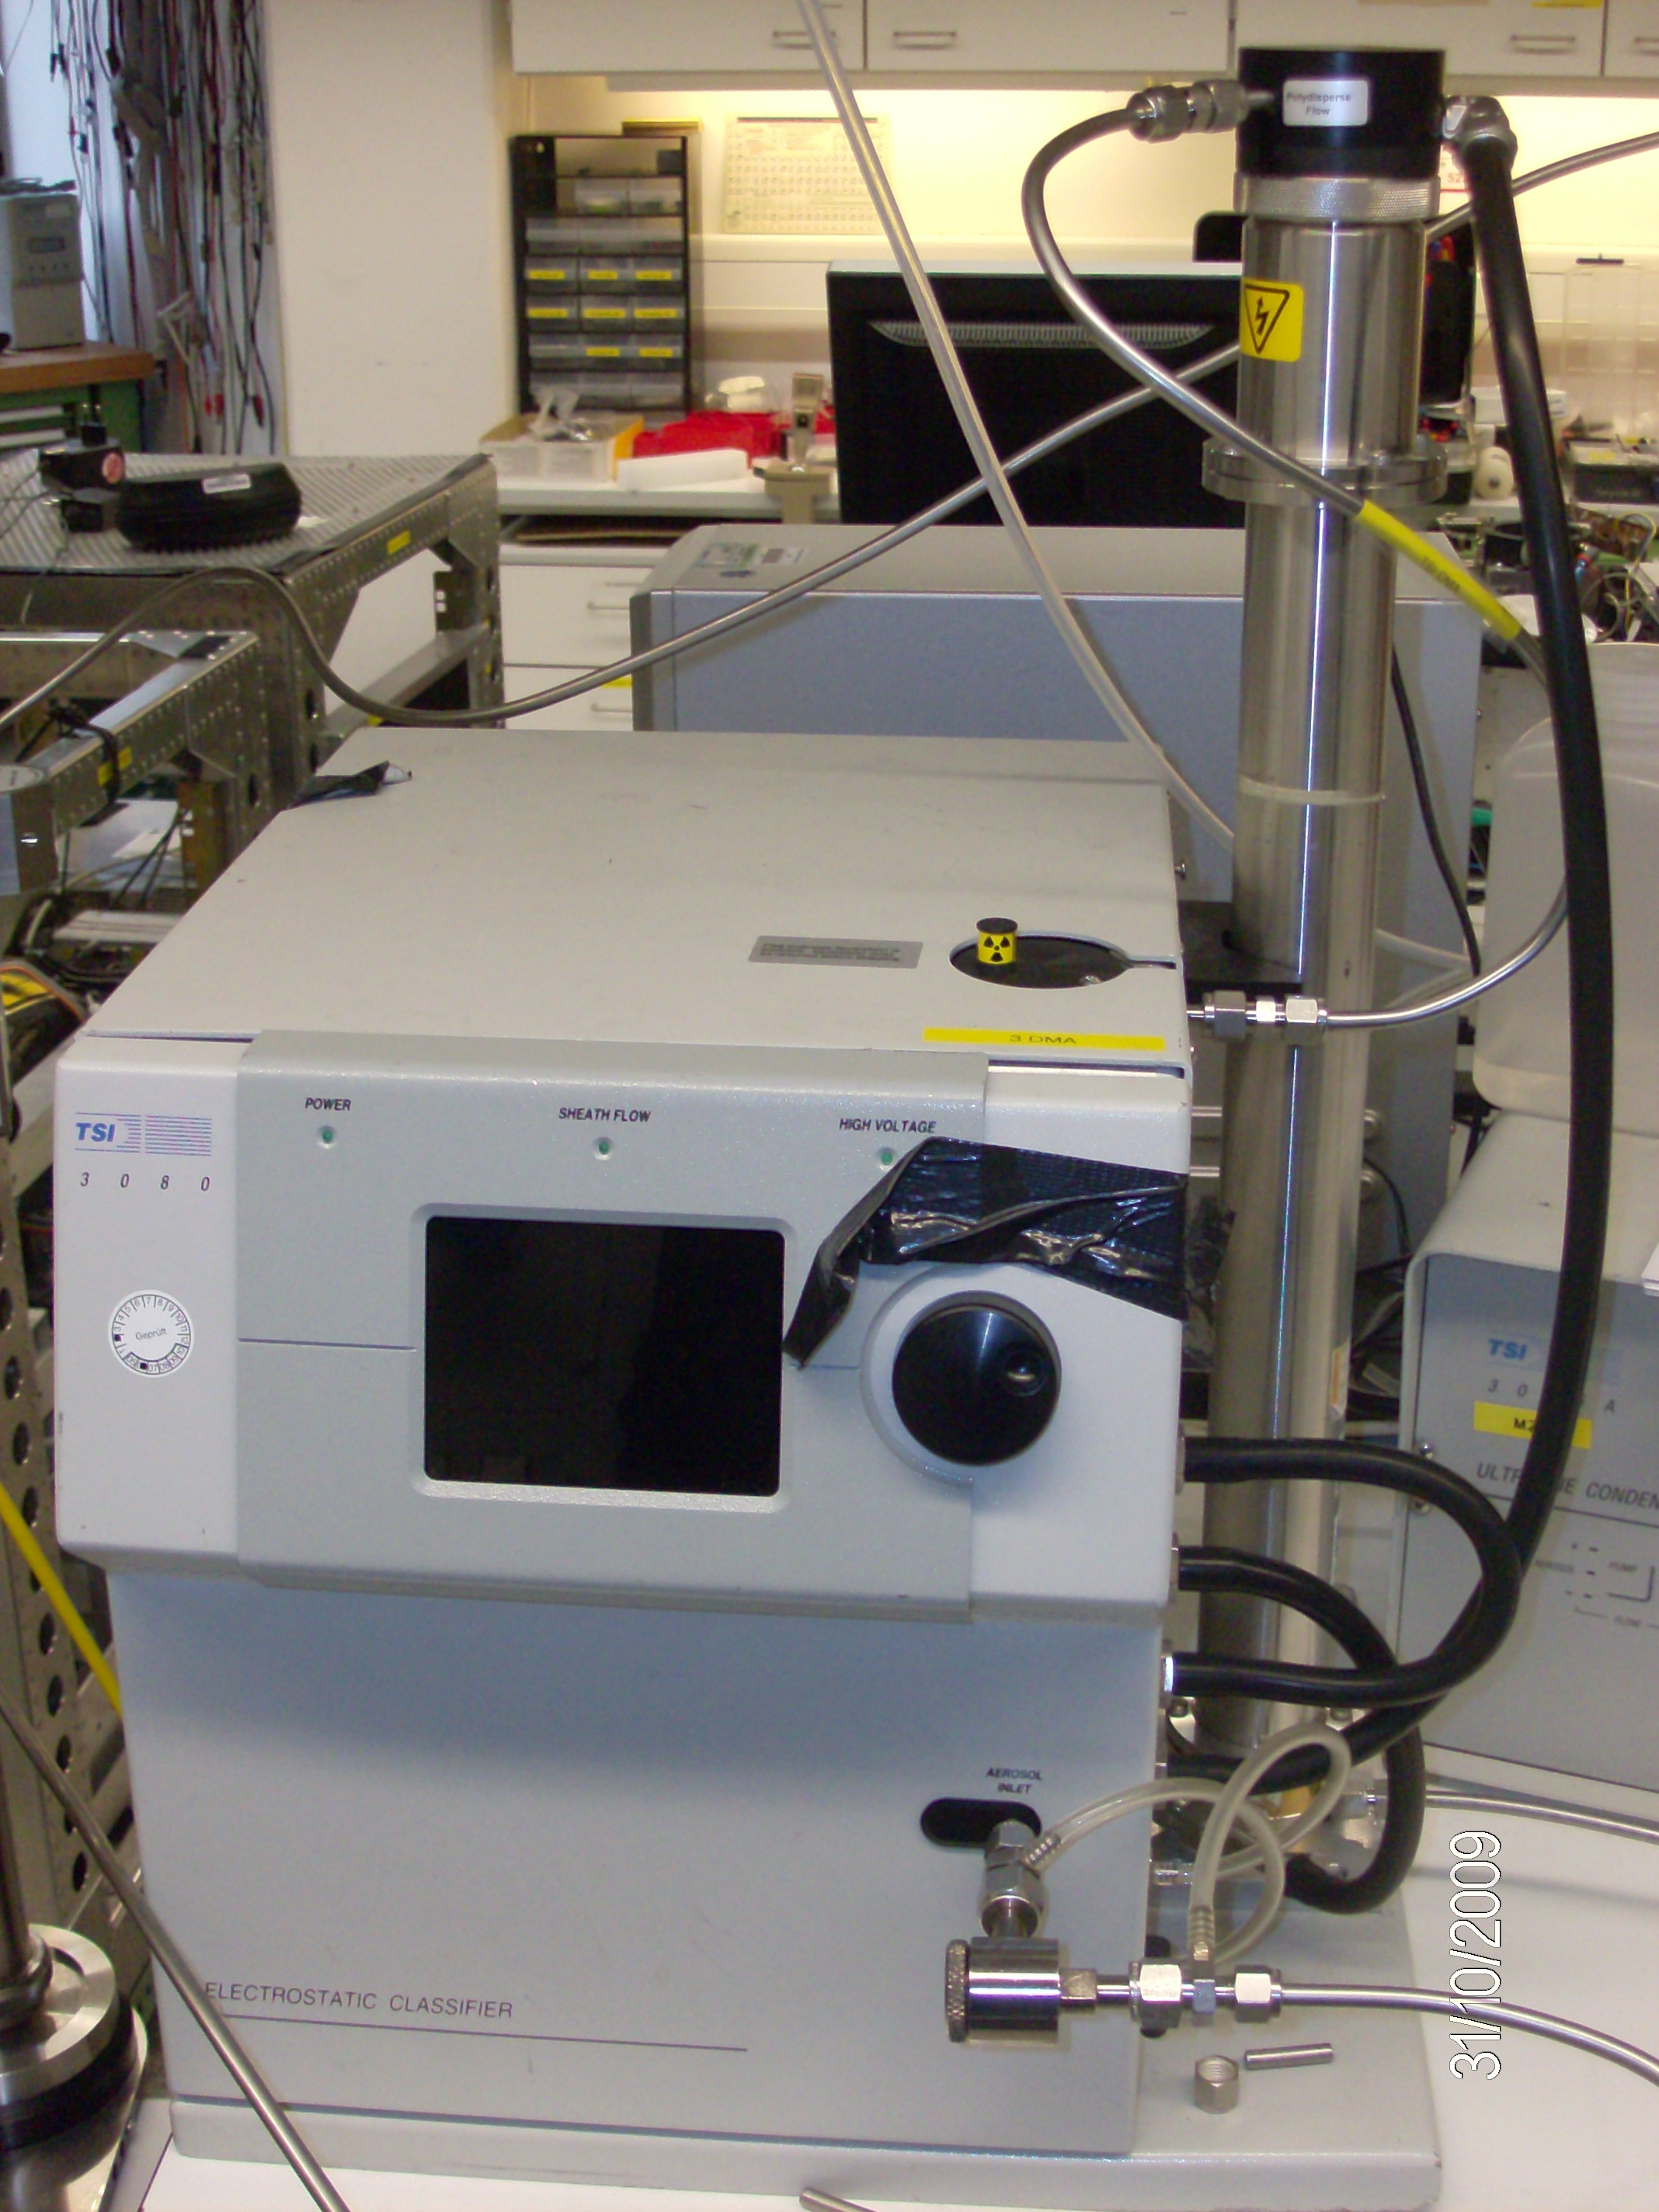
\includegraphics[scale=0.1]{eps/TSI3080CE.eps}\\
\end{center}
\caption{\label{TSI3080CE}\hspace{-0.1em} classificador eletrost\'{a}tico (TSI 3080).}
\end{figure}


\begin{figure}[hbt]
\begin{center}
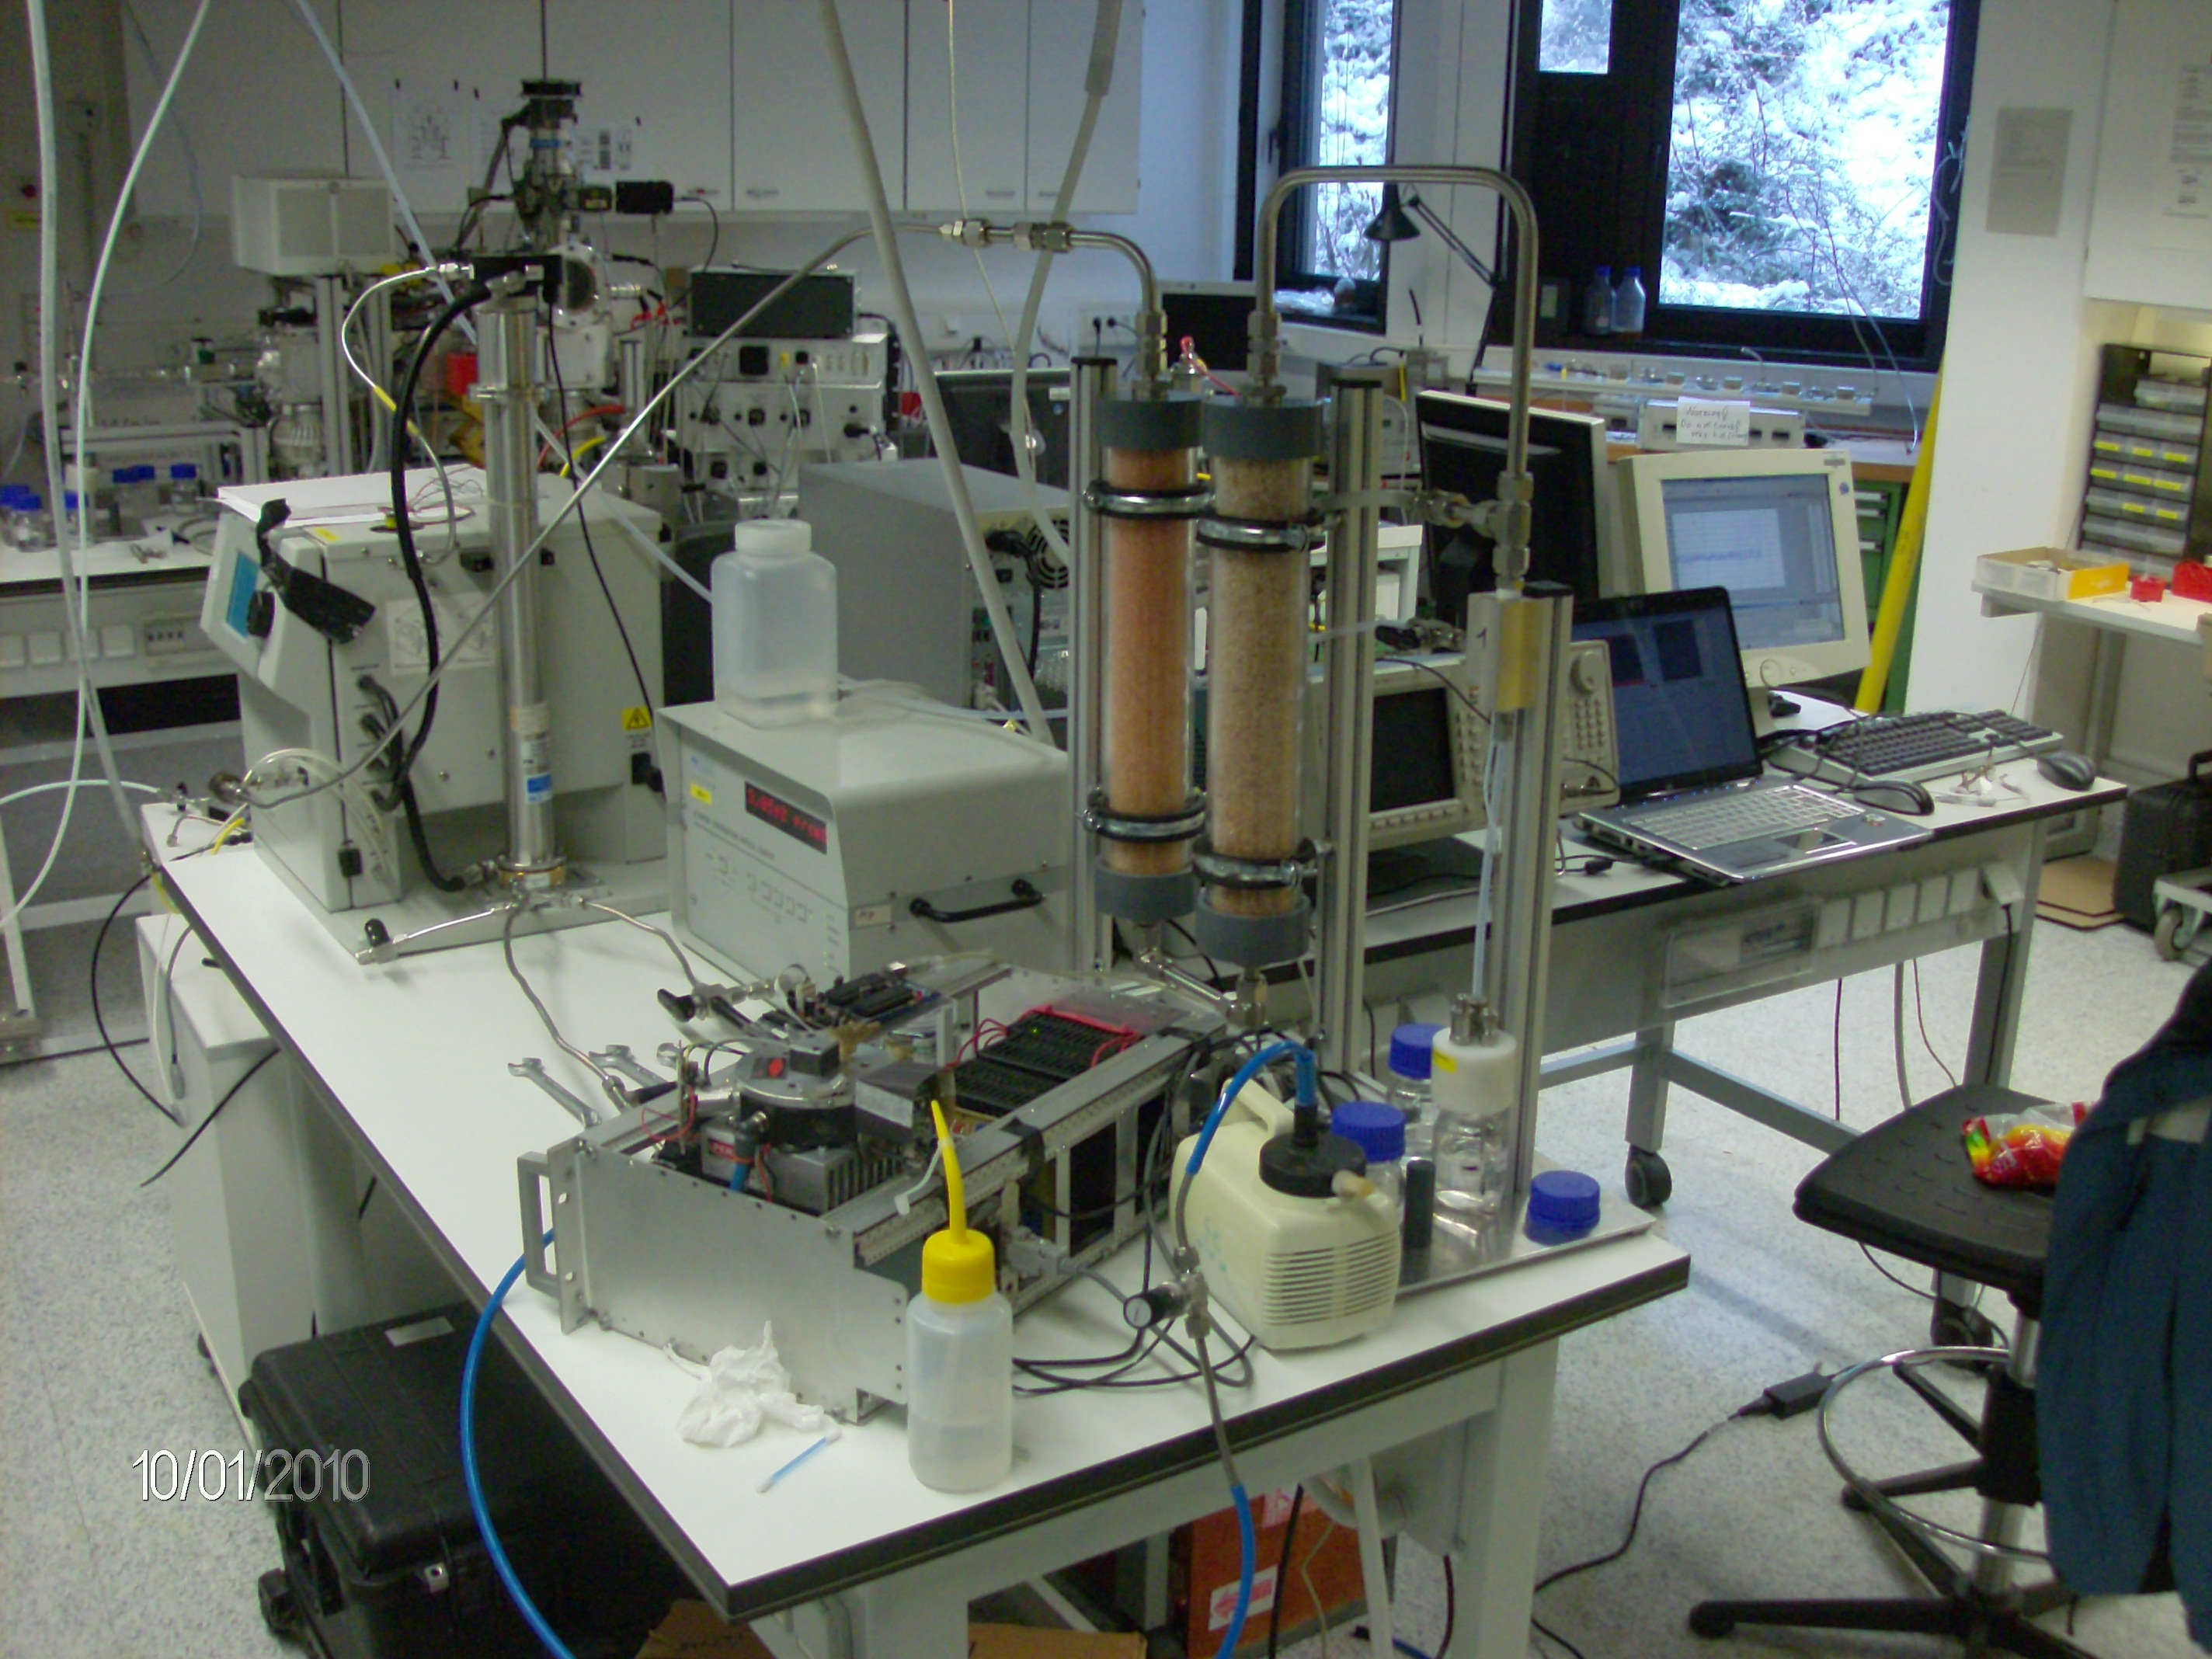
\includegraphics[scale=0.1]{eps/BANCADA_FOTO.eps}\\
\end{center}
\caption{\label{BANCADA_FOTO}\hspace{-0.1em} vista geral da bancada (TSI 3080).}
\end{figure}


\subsection{Prevenindo perda de part\'{\i}culas por deposi\c{c}\~{a}o eletrost\'{a}tica}
As medidas de aeross\'{o}is requerem um sistema de dutos para condu\c{c}\~{a}o destes aeross\'{o}is at\'{e} os mais variados instrumentos de medi\c{c}\~{a}o. Dependendo das caracter\'{\i}sticas f\'{\i}sicas dos aeross\'{o}is e dos dutos, diversos mecanismos de perda de part\'{\i}culas podem interferir nas medi\c{c}\~{o}es \cite{SL}. Uma destas causas chama-se de perda por deposi\c{c}\~{a}o eletrost\'{a}tica. Quando os aeross\'{o}is s\~{a}o produzidos em atomizadores, nebulizadores ou atrav\'{e}s de mecanismos naturais, alguns podem n\~{a}o estar eletricamente neutros. No caso destes aeross\'{o}is serem capturados pelos dutos de qualquer medidor de concentra\c{c}\~{a}o, pode ocorrer de algumas part\'{\i}culas ficarem retinas nos pr\'{o}prios dutos caso estes n\~{a}o sejam de material condutor e n\~{a}o estejam aterrados. Com o objetivo de verificar estas perdas, um experimento foi realizado e consistia em comparar a medida da concentra\c{c}\~{a}o realizada pelo CPC em 2 condi\c{c}\~{o}es: a primeira utilizando um duto coletor de 3 metros de pl\'{a}stico e a segunda utilizando um duto de a\c{c}o inox de mesmo comprimento. A medida foi realizada durante 50 segundos para cada caso. O resultado deste experimento mostrou que este efeito n\~{a}o pode ser negligenciado no caso de dutos longos, pois, a diferen\c{c}a chegou a 13\% na m\'{e}dia como \'{e} mostrado na Tabela \ref{perdas} e na Figura \ref{duto}.


\begin{table}[!htbp]
\centering \caption{\label{perdas} compara\c{c}\~{a}o entre concentra\c{c}\~{o}es medidas realizadas por dutos de a\c{c}o e pl\'{a}stico}
\begin{tabular}{ c | c  }
  \hline
  Tipo de duto & Concentra\c{c}\~{a}o m\'{e}dia\\
  \hline
  A\c{c}o & 2611\\
  Pl\'{a}stico & 2272\\
  \hline
  Diferen\c{c}a & 13 \% \\
  \hline
\end{tabular}\\
\end{table}



\begin{figure}[hbt]
\begin{center}
\includegraphics[scale=1.0]{eps/dutos.eps}\\
\end{center}
\caption{\label{duto}\hspace{-0.1em} perdas em fun\c{c}\~{a}o do tipo de duto. }
\end{figure}





    \include{ccnc_incertezas/ccnc_incertezas}
     \chapter{Diagrama el\'{e}trico do CCNC-SDCC}

\newpage
\begin{figure}[!hbt]
    \begin{center}
        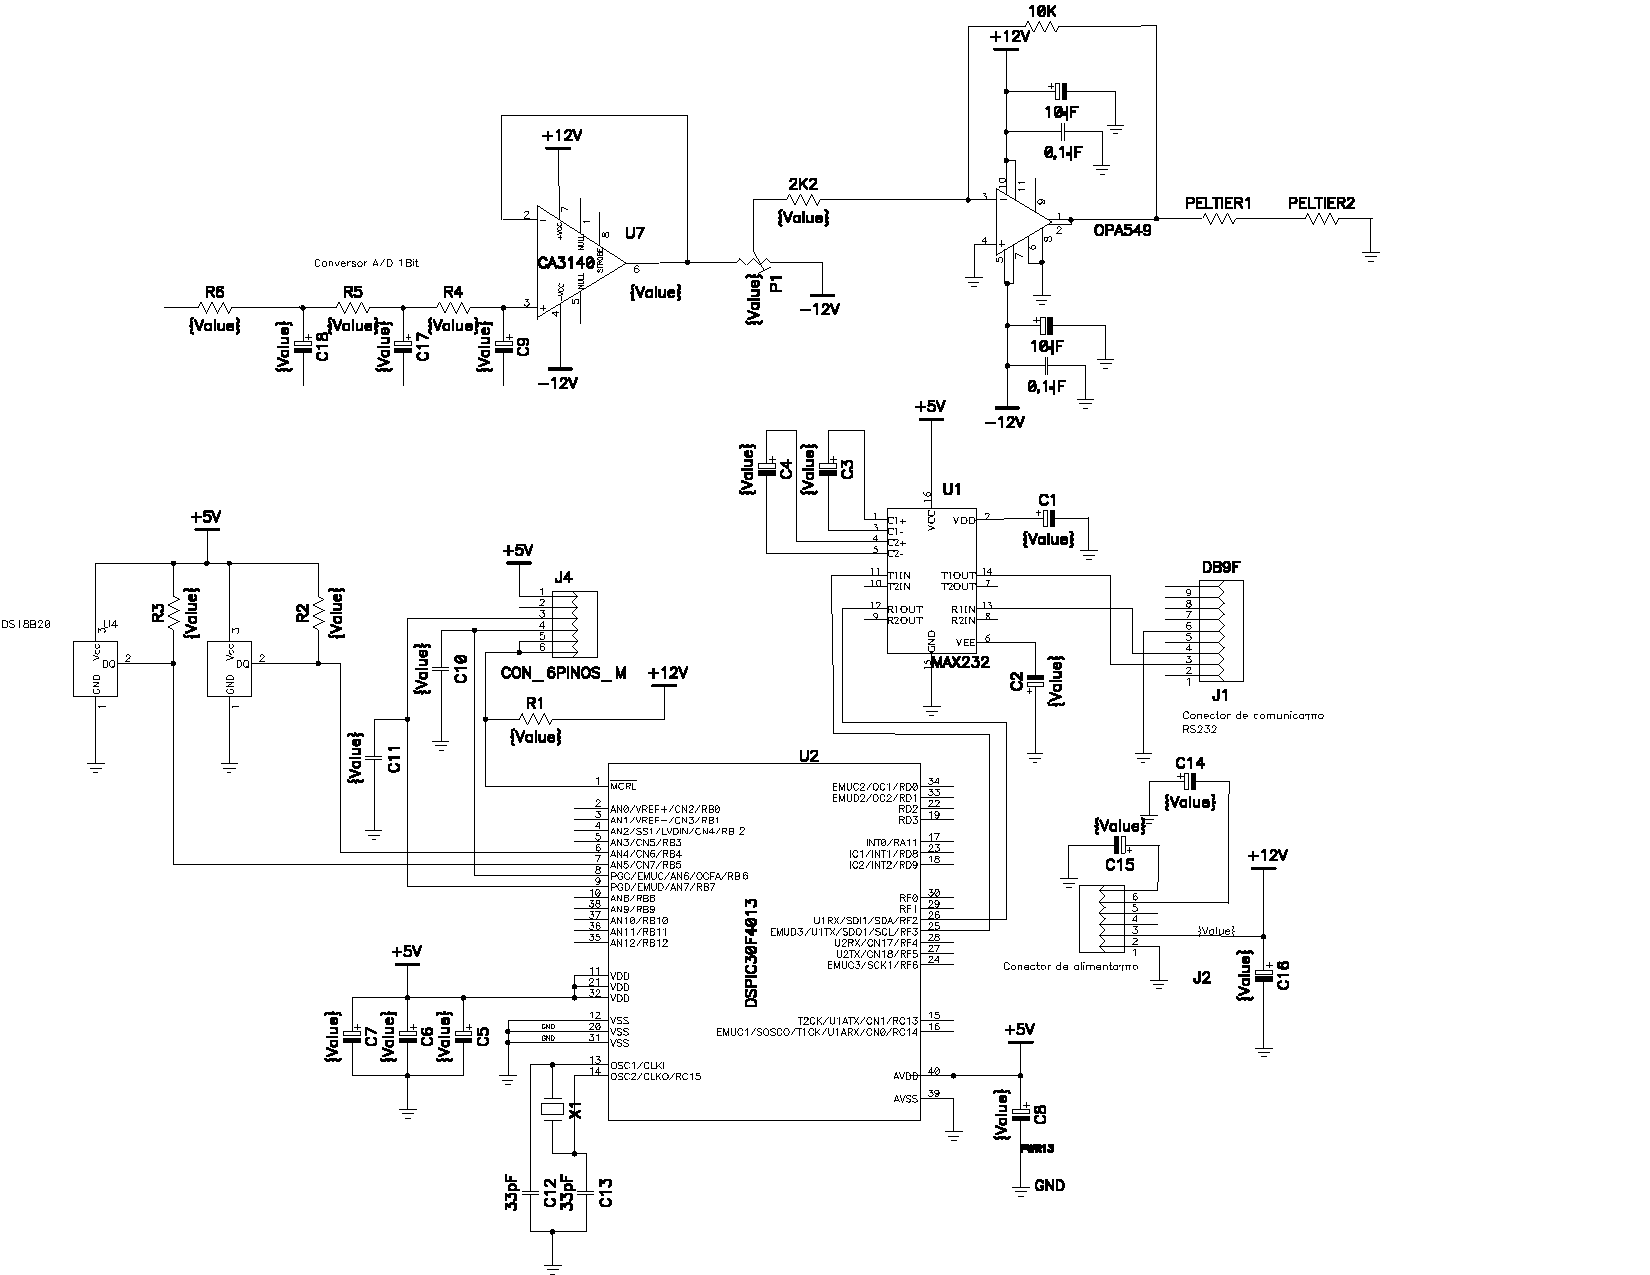
\includegraphics[bb=1.0in 12.0in 7.5in 10in,scale=0.9]{eps/ccncsch.pdf}
    \end{center}
    \caption{\label{ccncsch}\hspace{-0.1em} diagrama el\'{e}trico da unidade de controle do CCNC-SDCC.}
\end{figure}



\end{appendices}


%%%%%%%%%%%%%%%%%%%%%%%%%%%%%%%%%%%%%%%%%%%%%%%%%%%%%%%%%%%%%%%%%
%%%% INDICE REMISSIVO
%%%%%%%%%%%%%%%%%%%%%%%%%%%%%%%%%%%%%%%%%%%%%%%%%%%%%%%%%%%%%%%%%
%%%% GLOSS\'{A}RIO
%%%%%%%%%%%%%%%%%%%%%%%%%%%%%%%%%%%%%%%%%%%%%%%%%%%%%%%%%%%%%%%%%
%%%% REFER\^{E}NCIAS BIBLIOGR\'{A}FICAS
\bibliographystyle{abnt-alf}

\ifthenelse{\isundefined{\alfref}}{\bibliographystyle{unsrtnat}}{\bibliographystyle{abnt-alf}}
\bibliography{C:/Users/FGMPinheiro/Documents/refbib/ref_bib_fgmp}

\addcontentsline{toc}{chapter}{\bibname}

\end{document}
